\documentclass[c, 10pt]{beamer}

%\usepackage{tikz}
%\usetikzlibrary{backgrounds,fit, positioning,shapes}
\usepackage{mathtools}
\usepackage{xcolor}
\usepackage{colortbl}
\usepackage{rotating}
%\newlength{\NOTskip} 
%\def\NOT#1{\settowidth{\NOTskip}{\ensuremath{#1}}%
%	\hspace{0.5\NOTskip}\mathclap{\not}\hspace{-0.5\NOTskip}#1}
\usepackage{url}
\def\UrlBreaks{\do\/\do-}
\usepackage{caption}
\newcommand{\source}[1]{\caption*{\tiny Adapted from: {#1}} }
\usepackage[absolute,overlay]{textpos}


\usepackage{natbib}
\bibliographystyle{apalike}


\usecolortheme{orchid}
\mode<presentation>
{
	\usetheme{default}      % or try Darmstadt, Madrid, Warsaw, ...
	\usecolortheme{default} % or try albatross, beaver, crane, ...
	\usefonttheme{default}  % or try serif, structurebold, ...
	\setbeamertemplate{navigation symbols}{}
	\setbeamertemplate{caption}[numbered]
} 

\addtobeamertemplate{navigation symbols}{}{%
	\usebeamerfont{footline}%
	\usebeamercolor[fg]{footline}%
	\hspace{1em}%
	\insertframenumber/\inserttotalframenumber
}

\setbeamerfont{frametitle}{size=\LARGE}

\newcommand{\backupbegin}{
	\newcounter{framenumberappendix}
	\setcounter{framenumberappendix}{\value{framenumber}}
}
\newcommand{\backupend}{
	\addtocounter{framenumberappendix}{-\value{framenumber}}
	\addtocounter{framenumber}{\value{framenumberappendix}} 
}

\newsavebox{\authbox}
\sbox{\authbox}{%
	\centering
	\begin{minipage}{0.45\linewidth}
		\centering\normalsize
		\textit{Author}: \par
		Samuele Vianello
	\end{minipage}
	\hfill
	\begin{minipage}{0.45\linewidth}
		\centering\normalsize
		\textit{Supervisors}: \par
		Daniele Marazzina \\
		Ferdinando M. Ametrano
	\end{minipage}
}


\title{Bitcoin as a Digital Asset:}
\subtitle{Correlation and Optimal Portfolio Allocation}
\author[Samuele Vianello]{%
	\usebox{\authbox}
}

\bigskip

\institute{School of Industrial and Information Engineering \\
	Master of Science in Mathematical Engineering}
\date{16$^{\text{th}}$ April 2019}
\titlegraphic{%
	\begin{picture}(0,0)
	\put(30, 230){\makebox(0,0)[rt]{
\includegraphics[width=2cm]{Images/polimi.png}}}
	\end{picture}}

\setbeamertemplate{bibliography entry title}{}
\setbeamertemplate{bibliography entry location}{}

\begin{document}
	\AtBeginSection[]{
	\begin{frame}[noframenumbering]{Outline}
		\small \tableofcontents[currentsection, hideothersubsections]
	\end{frame} 
	}

    \begin{frame}
    	\bigskip
    	
    	\bigskip
    	\large
        \maketitle
    \end{frame}
	
	\begin{frame}{Objectives}
	The main goals of this work are the following:
		\begin{enumerate}
			\item Study the \textbf{correlation} of Bitcoin's returns with those of other standard assets by computing the \textit{sample} \textit{(Pearson's)} \textit{correlation}, performing tests on its \textit{significance} and computing the \textit{rolling correlations}.
			\item \textbf{Calibrate} three different continuous-time \textbf{models for the multivariate dynamics of the asset prices} (Merton, Heston and Bates) in order to obtain the levels of the correlation in a more sophisticated frameworks that includes \textit{jumps} and \textit{stochastic volatility}.
			\item Study the \textbf{optimal allocation} for a portfolio that contains Bitcoin and the \textbf{diversification properties} of the inclusion of the digital asset. 
		\end{enumerate}
	\end{frame}


\begin{frame}{Introduction}
Bitcoin was introduced in \citep{BTC2008} as a \textit{peer-to-peer} electronic cash system. It started off as a system that was only used by a niche of people in online cryptography forums but year by year it quickly gained notoriety.

\bigskip
Through its distributed blockchain, Bitcoin is able to solve the problem of double spending without the need for a trusted third party. Transaction are quickly validated by the network, making the transfer of wealth as easy as online data sharing.

\bigskip
Bitcoin's monetary policy based on deterministic supply achieves \textit{scarcity} in the digital realm and mimics the progressive scarcity of gold.
\end{frame}




\section{Dataset}

\begin{frame}[allowframebreaks]{Dataset}
\bigskip
The dataset is composed of 2163 observations of the prices of \textit{16 assets valued daily} (excluding holidays and weekends) from 19/07/2010 till 2/11/2018 (all data provided by Bloomberg).

The assets are grouped into five classes:

\begin{enumerate}
	\item \textbf{Bitcoin} (btc): Value of a single bitcoin, quoted in dollars.

	\item Stock indexes:
	\begin{itemize}
		\item \textbf{S\&P500} (sp500): American stock market index based on 500 large company with stock listed either on the NYSE or NASDAQ.
		\item \textbf{EUROSTOXX 50} (eurostoxx): equity index of eurozone stocks, covering 50 stocks from 11 eurozone countries.
		\item \textbf{MSCI BRIC} (bric): market cap weighted index designed to measure the equity market performance across the emerging country indexes of Brazil, Russia, India and China.
		\item \textbf{NASDAQ}(nasdaq): market cap weighted index including all NASDAQ tiers: Global Select, Global Market and Capital Market.
	\end{itemize}
	
	\framebreak
	
	\item Bond indexes:
	\begin{itemize}
		\item \textbf{BBG Pan European} (bond\_europe): Bloomberg Barclays Pan-European Aggregate Index that tracks fixed-rate, investment-grade securities issued in different European currencies.
		\item \textbf{BBG Pan US} (bond\_us): BBG US Aggregate Bond Index, a benchmark that measures investment grade, US dollar-denominated, fixed-rate taxable bond market.
		\item \textbf{BBG Pan EurAgg} (bond\_eur): similar to the Pan European but it only considers securities issued in Euros.
	\end{itemize} 
	\item Currencies:
	\begin{itemize}
		\item \textbf{EUR/USD} (eur): spot value of one Euro in  US dollars. 
		\item \textbf{GBP/USD} (gbp): spot value of one British Pound in US dollars.
		\item \textbf{CHF/USD} (chf): spot value of one Swiss Franc in  US dollars.
		\item \textbf{JPY/USD} (jpy): spot value of one Japanese Yen in  US dollars.
	\end{itemize}
	\framebreak
	\item Commodities:
	\begin{itemize}
		\item \textbf{Gold} (gold): price of gold measured in USD/Oz.
		\item \textbf{WTI} (wti): price of crude oil used as benchmark in oil pricing and as the underlying commodity in the NYMEX oil future contracts.
		\item \textbf{Grain} (grain): S\&P GPSCI index that measures the performance of the grain commodity market.
		\item \textbf{Metals} (metal): S\&P GSCI Industrial Metals index that measures the movements of industrial metal prices including aluminium, copper, zinc, nickel and lead.
	\end{itemize}
\end{enumerate}
\end{frame}

\section{Correlation Analysis}

\begin{frame}{Empirical Correlation }
The empirical correlation is computed using Pearson's sample correlation formula on the daily log-returns obtained from the price dataset.
\begin{figure}
	\centering
     \noindent\makebox[\textwidth]{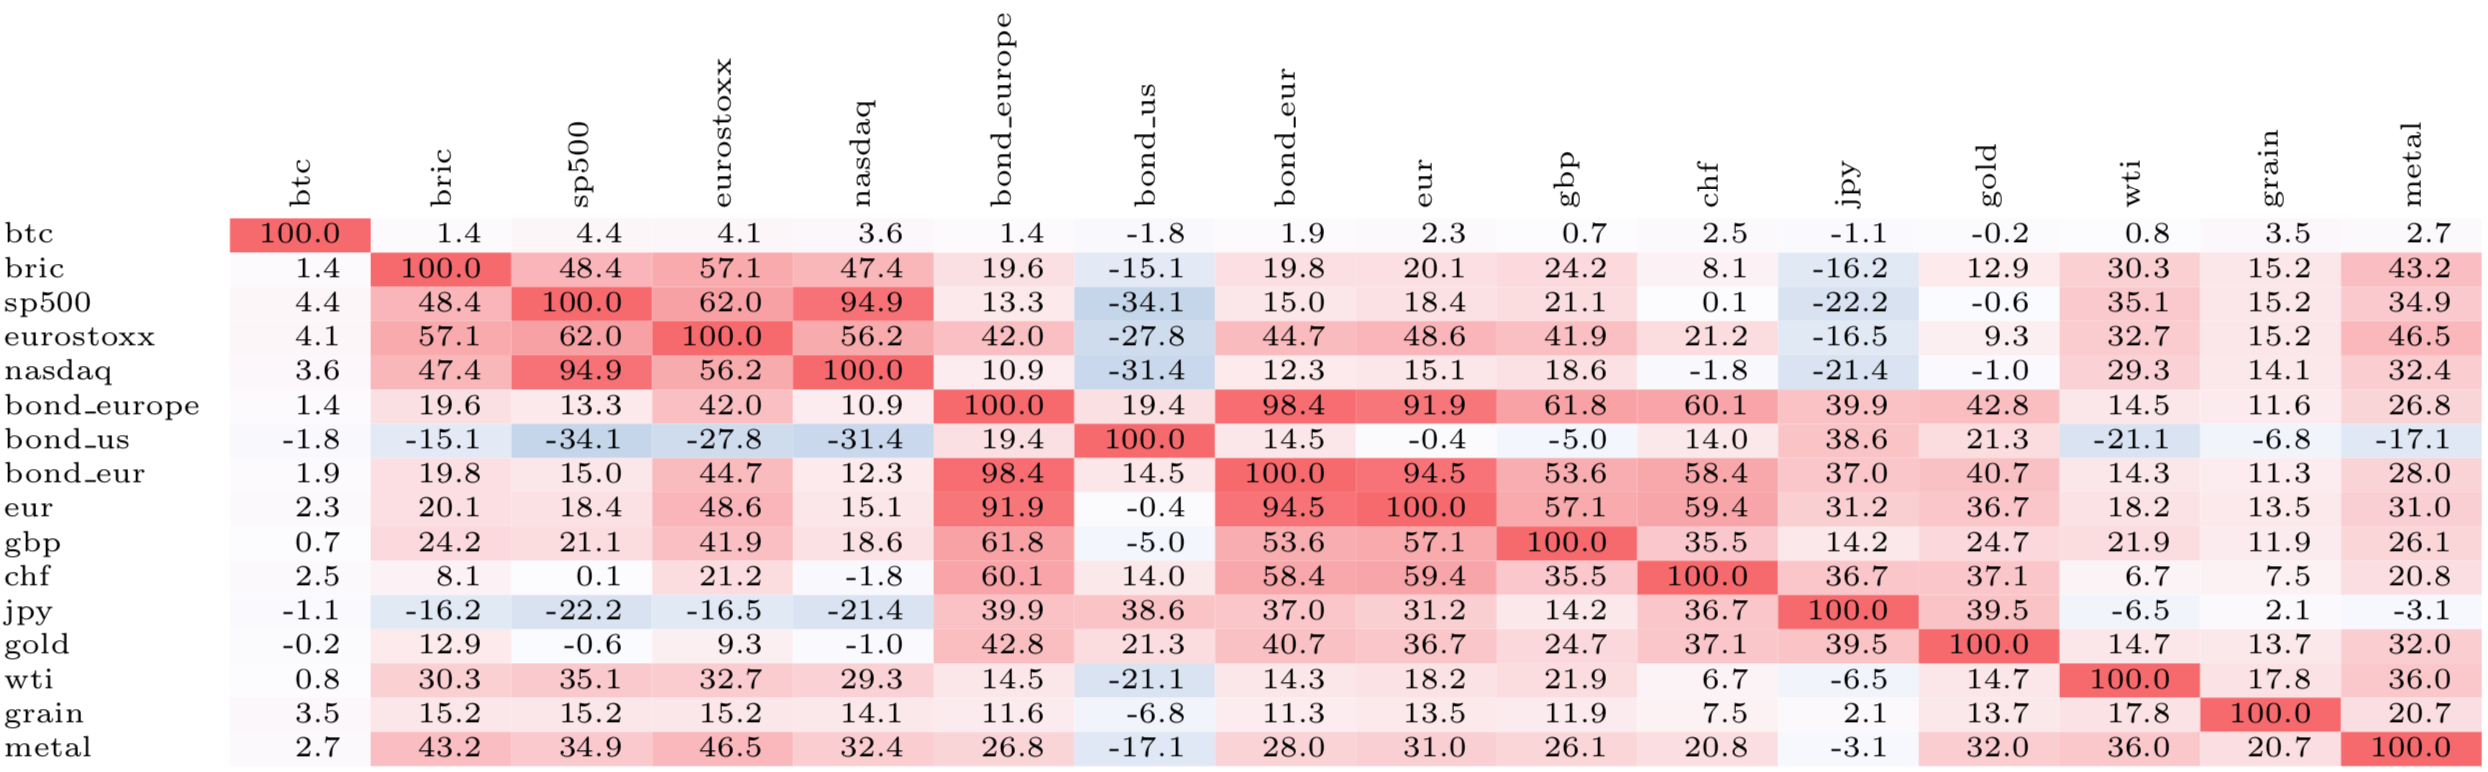
\includegraphics[width =1.1\textwidth]{Images/empirical_correlation}
    }
\end{figure}

The results clearly show that:
\begin{itemize}
	\item Bitcoin has \textbf{low correlation} with every asset.
	\item Assets in the same class usually have a \textbf{high correlation} among them.
\end{itemize}
\end{frame}


\begin{frame}{Correlation Significance}
	We perform two tests on the significance of the correlation between Bitcoin and each of the other assets, both of which investigate the following hypotheses:

	\begin{equation*}
	\mathbf{H_{0}}: \quad \rho = 0 \quad vs. \quad	\mathbf{H_{1}}: \quad \rho \neq 0 .
	\end{equation*}
	\textbf{Pearson's Test}: by computing \textit{Pearson's  t-statistic}, which under the null hypothesis is distributed as a Student's $t$, we can obtain the \textit{p-value} of the test and compare it to the confidence level of 95\%.
	
	\bigskip
	\textbf{Permutation test}: by permuting the sample of a pair of asset and computing Pearson's correlation on the permuted data a large number of times, we can reconstruct an empirical distribution for the possible correlations. Once we obtained this distribution, we can compute the \textit{p-value} of the test and compare it to the chosen confidence level.
\end{frame}
	

\begin{frame}{Correlation Significance}


\end{frame}




\section{Models Presentation and Calibration}



\section{Optimal Portfolio Allocation}


%    \section{Mathematical background and cryptographic primitives}
%    
%    \subsection{Hash functions}
%    \begin{frame}{Hash functions ($\simeq$ Random oracles)}
%    		\begin{center}
%    			\begin{tikzpicture}[
%    			every node/.style = {% is not necessary, default node's shape is rectangle
%    				align=center}
%    			]
%    			\tikzstyle{bigbox} = [draw=blue!50, thick, fill=blue!10, rounded corners, rectangle]
%    			\tikzstyle{box} = [minimum size=0.6cm, rounded corners,rectangle, fill=blue!50]
%    			
%    			\node (title1) [draw] {Input};
%    			
%    			\node (a) [below=of title1, yshift=0.5cm] {``Politecnico \\ di Milano"};
%    			\node (b) [below=of a, yshift=0.5cm] {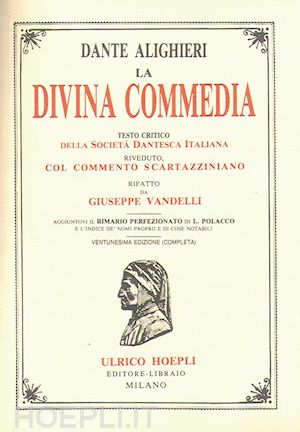
\includegraphics[scale=0.2]{Images/divina.jpg}};
%    			\node (c) [below=of b, yshift=0.5cm] {
\includegraphics[scale=0.07]{Images/film.jpg}};
%    			
%    			\begin{pgfonlayer}{background}
%    			\node[bigbox] [fit = (a) (c)] {};
%    			\end{pgfonlayer}
%    			
%    			\node[xshift=3.4cm] (title2) [draw, right=of title1] {Output};
%    			
%    			\node (d) [draw, right=of a, xshift = 0.5cm] {52c61456bd3d60c08599a8c61e113e7b \\ c39118b75d06b2643c55957ece91269b};
%    			\node (e) [draw, right=of b, xshift=0.7cm] {1f12f8384d5941e8e273926635be646a \\ f786405a8662e0ba6dd1fd0526ec0528};
%    			\node (f) [draw, right=of c, xshift=0.3cm] {721a14d89cb463b51cf20ecc707aa290 \\ 5b7c8f32d9114dc19fe353e611494bf1};
%    			
%    			\begin{pgfonlayer}{background}
%    			\node[bigbox] [fit = (d) (f)] {};
%    			\end{pgfonlayer}
%    			
%
%    			\node[xshift=1.9cm, yshift=-1.2cm] (z) {$\xrightarrow{\ \ \ \ \ \ \ \ \ \ \ }{}$};
%    			\node[xshift=1.8cm, yshift=-1.5cm] (z) {$\NOT{\xleftarrow{\ \ \ \ \ \ \ \ \ \ \ }}{}$};
%    			\node[xshift=1.8cm, yshift=-3.4cm] (z) {$\xrightarrow{\ \ \ \ \ \ \ \ \ \ \ \ }{}$};
%    			\node[xshift=1.7cm, yshift=-3.7cm] (z) {$\NOT{\xleftarrow{\ \ \ \ \ \ \ \ \ \ \ \ }}{}$};
%    			\node[xshift=2cm, yshift=-6.2cm] (z) {$\xrightarrow{\ \ \ \ \ \ \ \ \ }{}$};
%    			\node[xshift=1.9cm, yshift=-6.5cm] (z) {$\NOT{\xleftarrow{\ \ \ \ \ \ \ \ \ }}{}$};
%
%    			
%    			\node (g) [right=of d, xshift = -0.9cm] {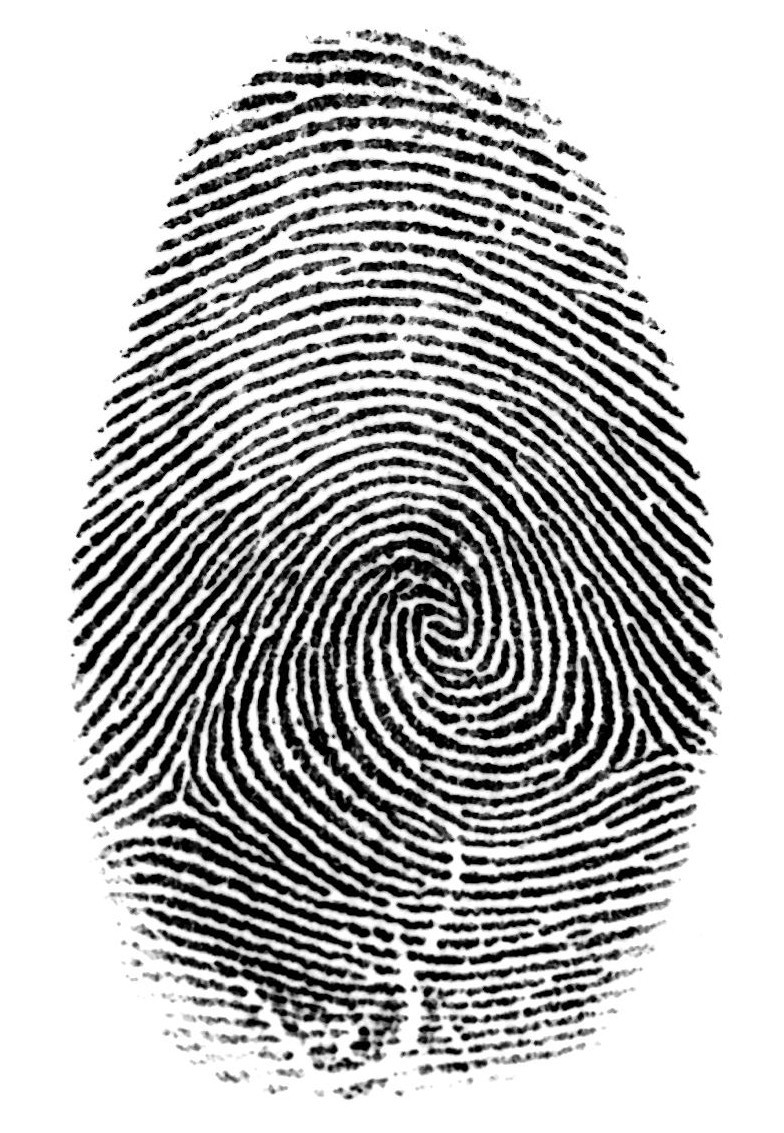
\includegraphics[scale=0.14]{Images/fingerprint1.jpg}};
%    			\node (g) [right=of e, xshift = -0.7cm] {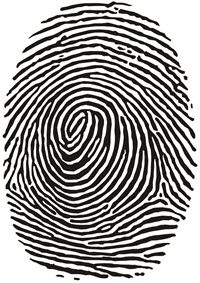
\includegraphics[scale=0.24]{Images/fingerprint2.jpg}};
%    			\node (g) [right=of f, xshift = -0.8cm] {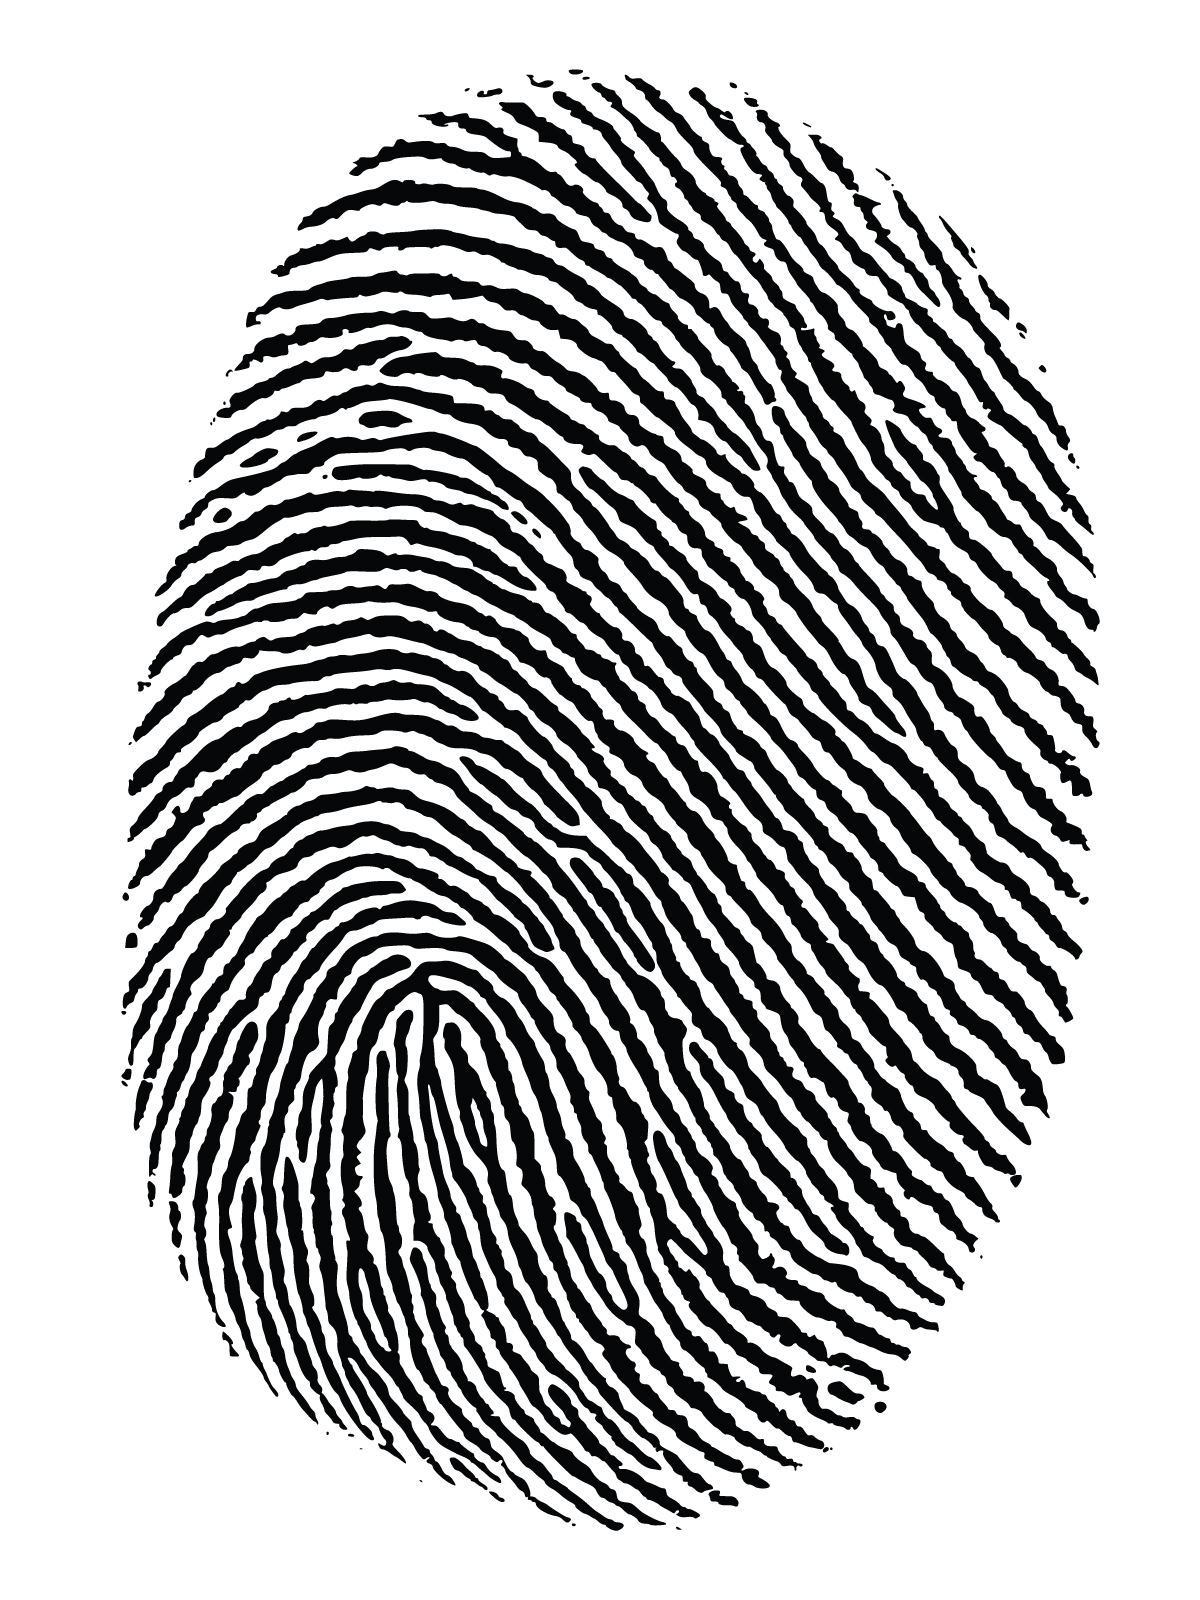
\includegraphics[scale=0.02]{Images/fingerprint3.jpg}};
%    			
%    			\node (h) [right=of a, xshift = -0.7cm, yshift = 0.3cm] {\tiny SHA-256};
%    			\node (h) [right=of b, xshift = -0.5cm, yshift = 0.3cm] {\tiny SHA-256};
%    			\node (h) [right=of c, xshift = -0.95cm, yshift = 0.3cm] {\tiny SHA-256};
%    			\end{tikzpicture}
%    		\end{center}
%		\end{frame}
%
%		\subsection{Elliptic curve cryptography}
%		\begin{frame}{Elliptic curve cryptography}
%			\begin{columns}
%				\begin{column}{0.5\linewidth}
%					An elliptic curve over a finite field is defined by the equation: 
%					$$E: \ y^2 = x^3 + ax + b \ (\text{mod} \ p).$$
%					Bitcoin: $a = 0, b = 7, p \simeq 2^{256}$.
%					
%					\bigskip
%					\noindent
%					It is possible to define:
%					\begin{itemize}
%						\item \hyperlink{point_addition}{Addition}: \\
%						$Q_3 := Q_1 + Q_2,$ 
%						\\$\forall Q_1, Q_2 \in E$;
%						\item Scalar multiplication: \\
%						$qG := G + ... + G$, $\forall G \in E,$ $\forall q \in \mathbb{N}$.
%					\end{itemize}
%			\end{column}
%			\begin{column}{0.6\linewidth}
%				\begin{tikzpicture}[
%					every node/.style = {% is not necessary, default node's shape is rectangle
%					align=center}
%					]
%				
%					\node () at (0,0) {};
%					\node (a) [xshift = 2.3cm] {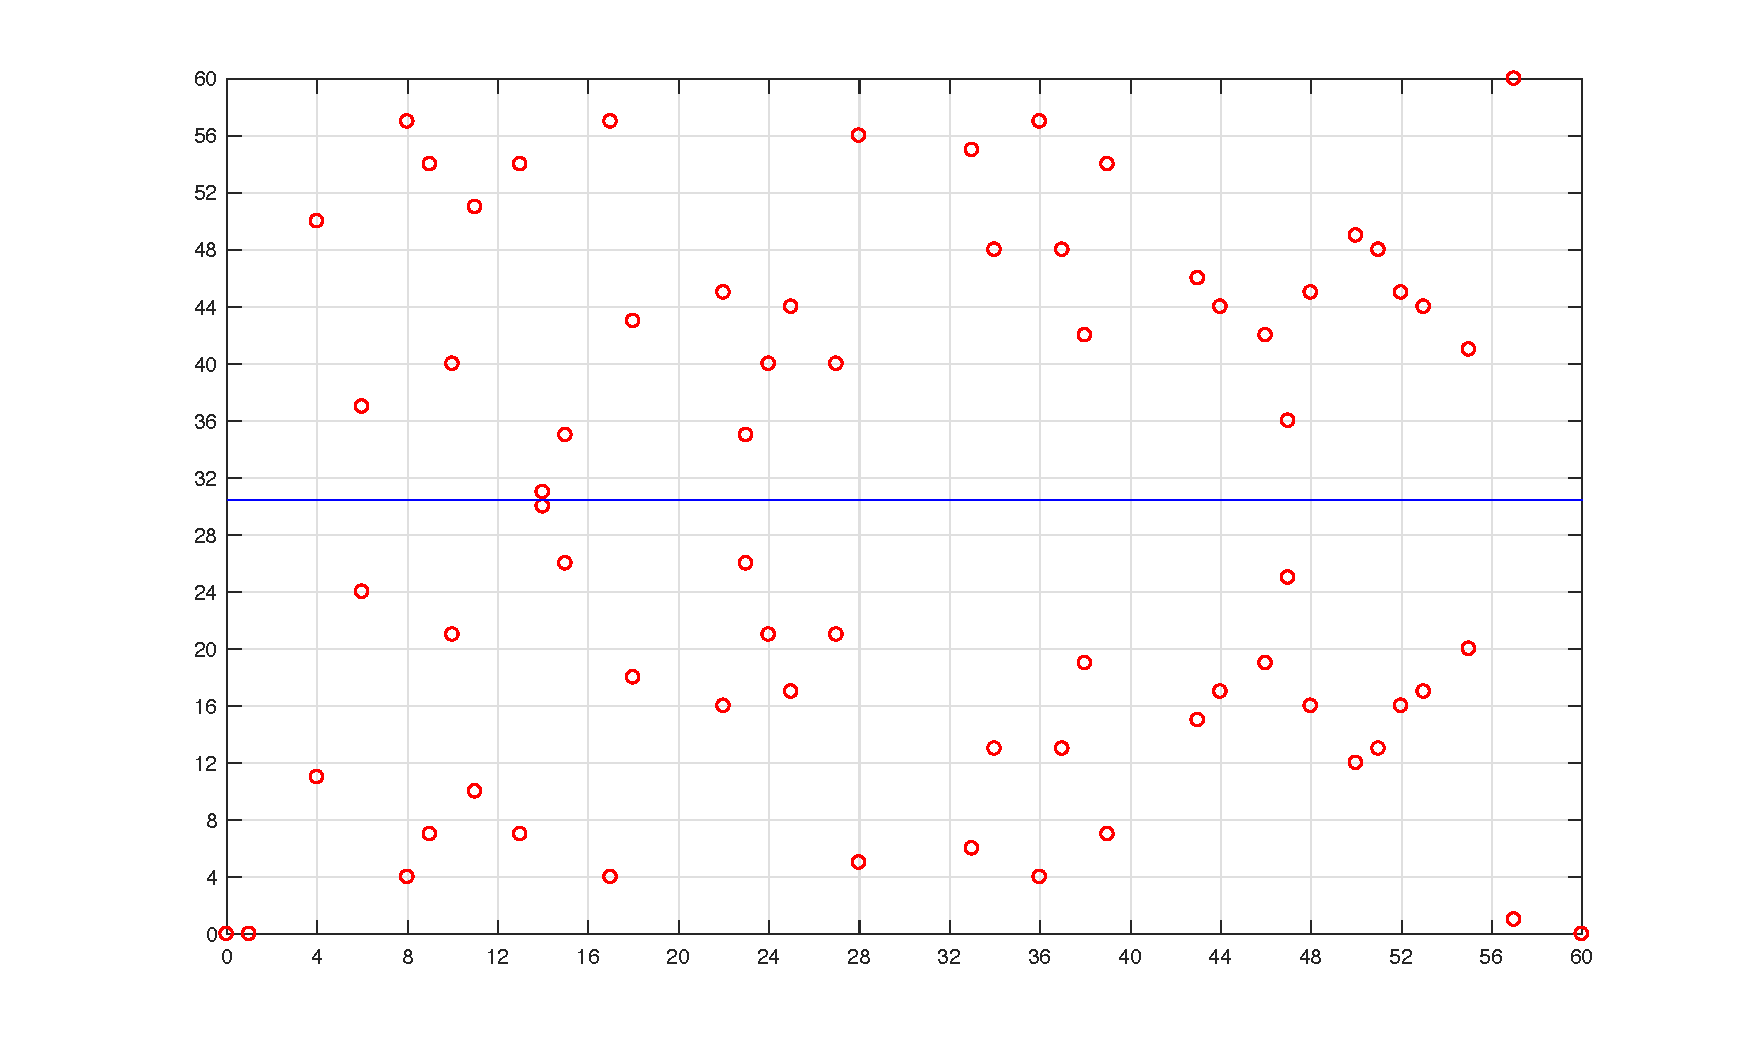
\includegraphics[height=5cm, width=6.4cm]{Images/ec_over_ff}};
%				
%					\node (b) [below=of a, yshift = 1.2cm] {\small The curve $y^2 = x^3 - x \ \text{over} \ \mathbb{F}_{61}$.};
%				\end{tikzpicture}
%			\end{column}
%		\end{columns}
%	\end{frame}
%
%    
%    \begin{frame}{Discrete logarithm problem}
%    	Fixed $G \in E$, we can define $Q = qG \ \ \forall q \in \{1, ..., n - 1\}$,  where $n$ is the smallest integer such that $nG = \infty$, the identity element of the sum:
%    	\begin{itemize}
%    		\item The direct operation $q \mapsto Q$ is efficient (\hyperlink{double_add}{double and add algorithm});
%    		\item The inverse operation $Q \mapsto q$ is computationally infeasible for certain groups.
%    	\end{itemize}
%    	
%    	\bigskip
%    	\noindent
%    	Asymmetric cryptography: $\{\textcolor{red}{q}, \textcolor{green}{Q}\}$ is a key pair whose elements have complementary roles.
%    	\begin{itemize}
%    		\item $\textcolor{red}{q}$: private key (signature);
%    		\item $\textcolor{green}{Q}$: public key (verification).
%    	\end{itemize}
%	\end{frame}
%    
%    \section{Digital signature schemes}
%    
%    \begin{frame}{Digital signature}
%        \begin{center}
%        	\begin{tikzpicture}[
%        	every node/.style = {% is not necessary, default node's shape is rectangle
%        		align=center}
%        	]
%        	
%        	\node (a) {
\includegraphics[scale=0.2]{Images/Alice.jpg}};
%        	\node (b) [text width=3cm, below=of a, yshift=1cm] {Alice};
%        	
%        	\node (d) [right=of a] {
\includegraphics[scale=0.25]{Images/Bob.jpg}};
%        	\node (e) [text width=3cm, below=of d, yshift=1cm] {Bob};
%        	
%        	\node<1-4> (c) [xshift=2.1 cm, yshift=-1cm] {
\includegraphics[scale=0.1]{Images/sig.jpg}};
%        	\node<1> (f) [xshift = 2.1 cm, yshift = 1cm] {
\includegraphics[scale=0.055]{Images/doc.png}};
%        	\node<2-> (f) [xshift = 2.1 cm, yshift = 1cm] {
\includegraphics[scale=0.1]{Images/bitcoin.png}};
%        	\node<5> (c) [xshift=2.1 cm, yshift=-1cm] {
\includegraphics[scale=0.1]{Images/bitcoin_sig.jpg}};
%
%        	
%        	\node<3> (f) [xshift = -1.2 cm, yshift = 1cm] {$q_A$};
%        	\node<3> (f) [xshift = 5.5 cm, yshift = 1cm] {$Q_A$};
%        	\node<4-> (f) [xshift = -1.2 cm, yshift = 1cm] {\textcolor{red}{$q_A$}};
%        	\node<4-> (f) [xshift = 5.5 cm, yshift = 1cm] {\textcolor{green}{$Q_A$}};
%        	
%        	
%        	
%        	
%        	\draw [->] (a) -- (d);
%        	\end{tikzpicture}
%        	\begin{itemize}
%        		\item<3-> Authentication: the recipient is confident that the funds come from the owner;
%        		\item<4-> Non repudiation: the sender cannot deny having sent the funds;
%        		\item<5> Integrity: ensures that the transaction has not been altered during transmission.
%        	\end{itemize}
%        \end{center}
%    \end{frame}
%
%	\subsection{ECDSA}
%	\begin{frame}{Elliptic curve digital signature algorithm}
%		\begin{columns}
%			\begin{column}{0.6\linewidth}
%				ECDSA\_SIG$(m, q)$:
%				\begin{enumerate}
%					\item<3 -> $k \xleftarrow{\text{\$}} \{1, ..., n - 1\}$;
%					\item<4 -> $K \gets kG$;
%					\item<5 -> $r \gets x_K \ (\text{mod} \ n)$;
%					\item<6-> $e \gets \text{hash}(m)$;
%					\item<7 -> $s \gets k^{-1}(e + rq) \ (\text{mod} \ n)$;
%					\item<8 -> \textbf{return} $(r, s)$.
%				\end{enumerate}
%			\end{column}
%			\begin{column}{0.5\linewidth}
%				\begin{figure}
%				\only<1> {\vspace*{-0.5cm}
%					\hspace*{-1cm}
%					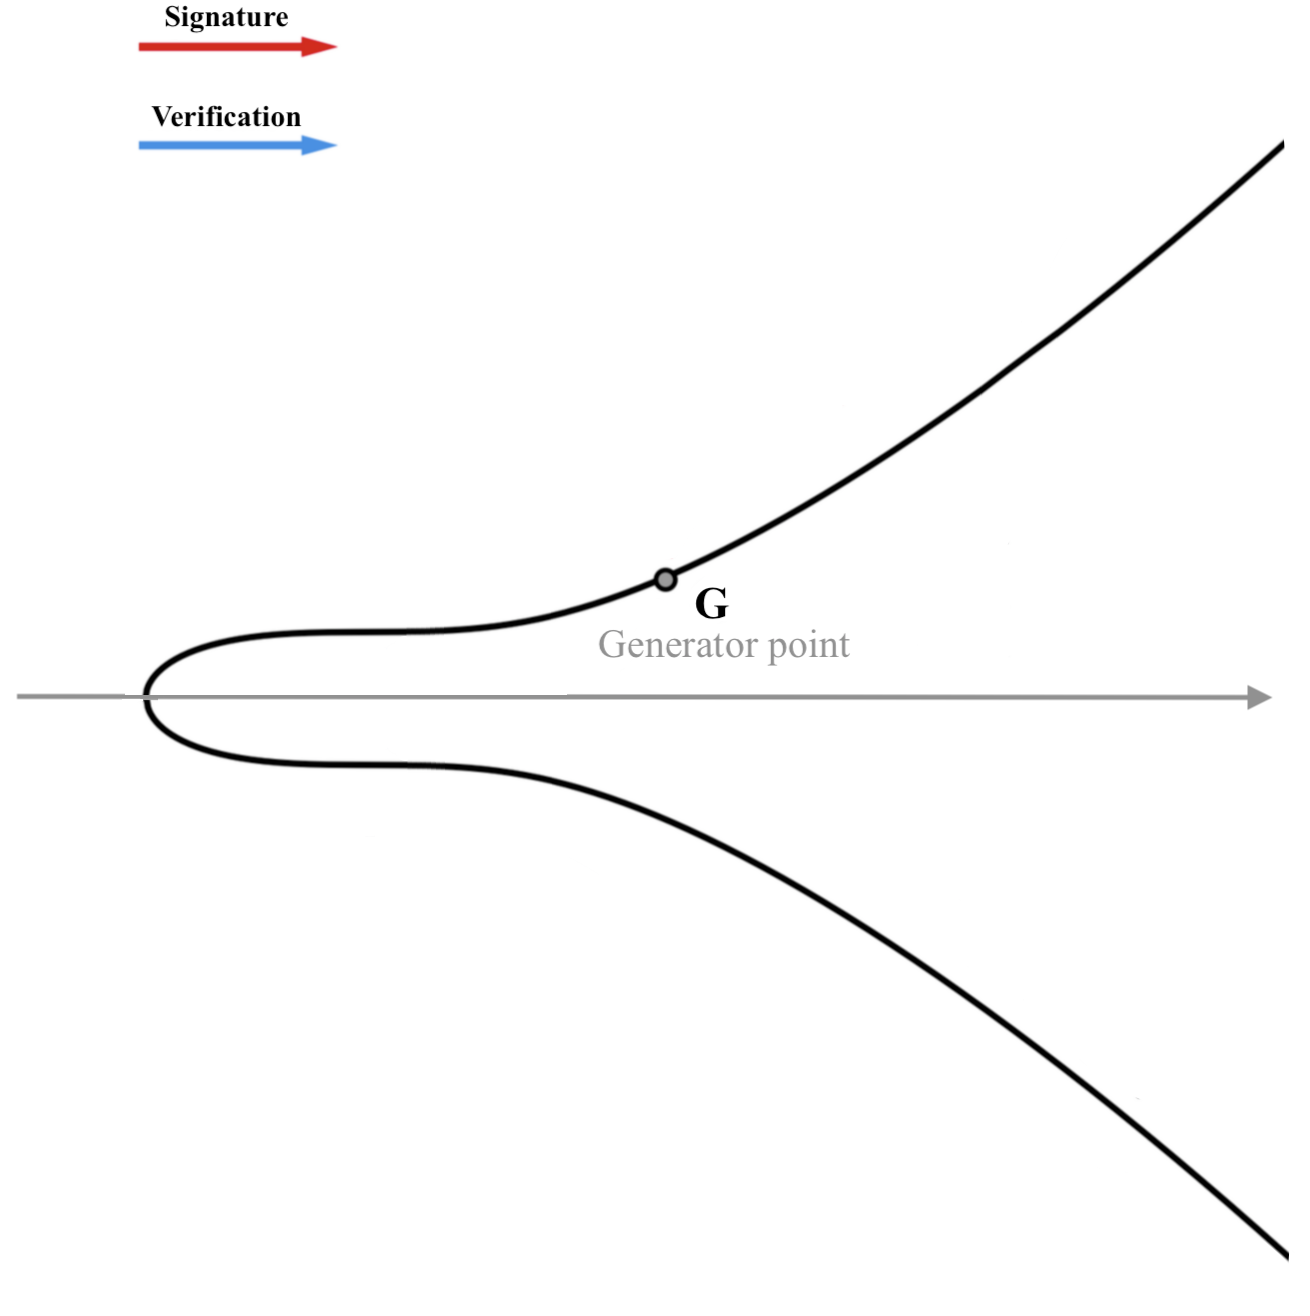
\includegraphics[scale=0.29]{Images/ECDSA1}
%				\source{\tiny \url{https://medium.com/cryptoadvance/how-schnorr-signatures-may-improve-bitcoin-91655bcb4744}}}
%				\only<2-3>{\vspace*{-0.5cm}
%					\hspace*{-1cm}
%					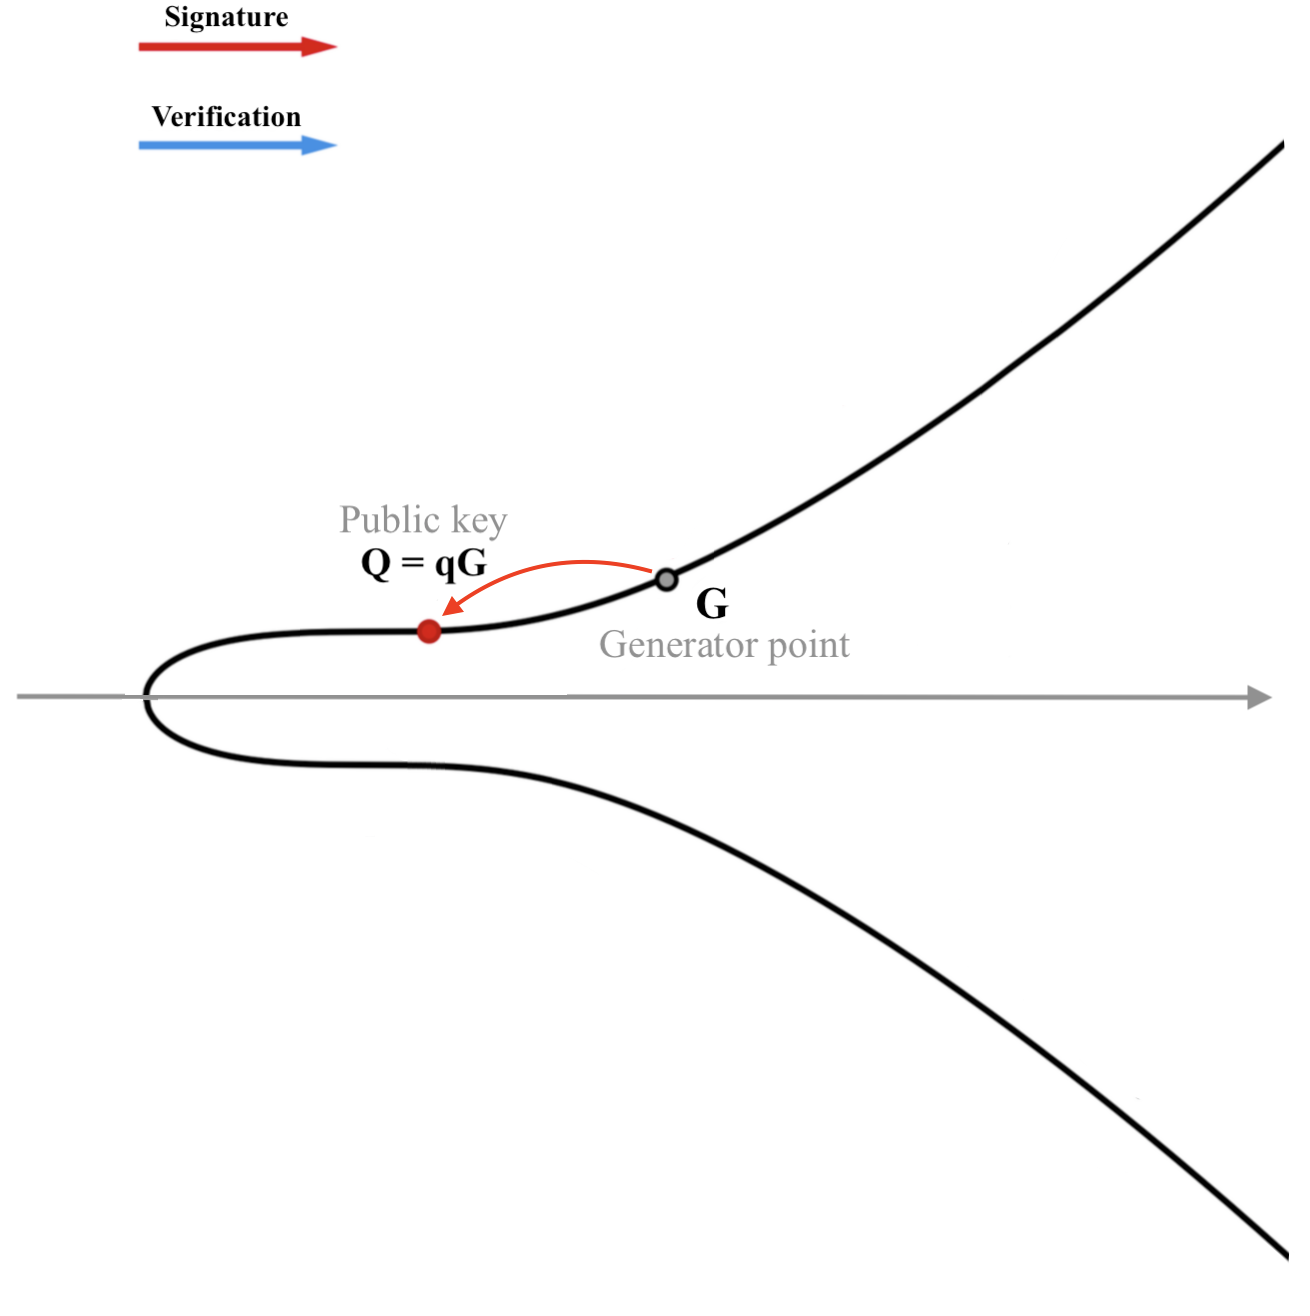
\includegraphics[scale=0.29]{Images/ECDSA2}
%				\source{\tiny \url{https://medium.com/cryptoadvance/how-schnorr-signatures-may-improve-bitcoin-91655bcb4744}}}
%				\only<4> {\vspace*{-0.5cm}
%					\hspace*{-1cm}
%					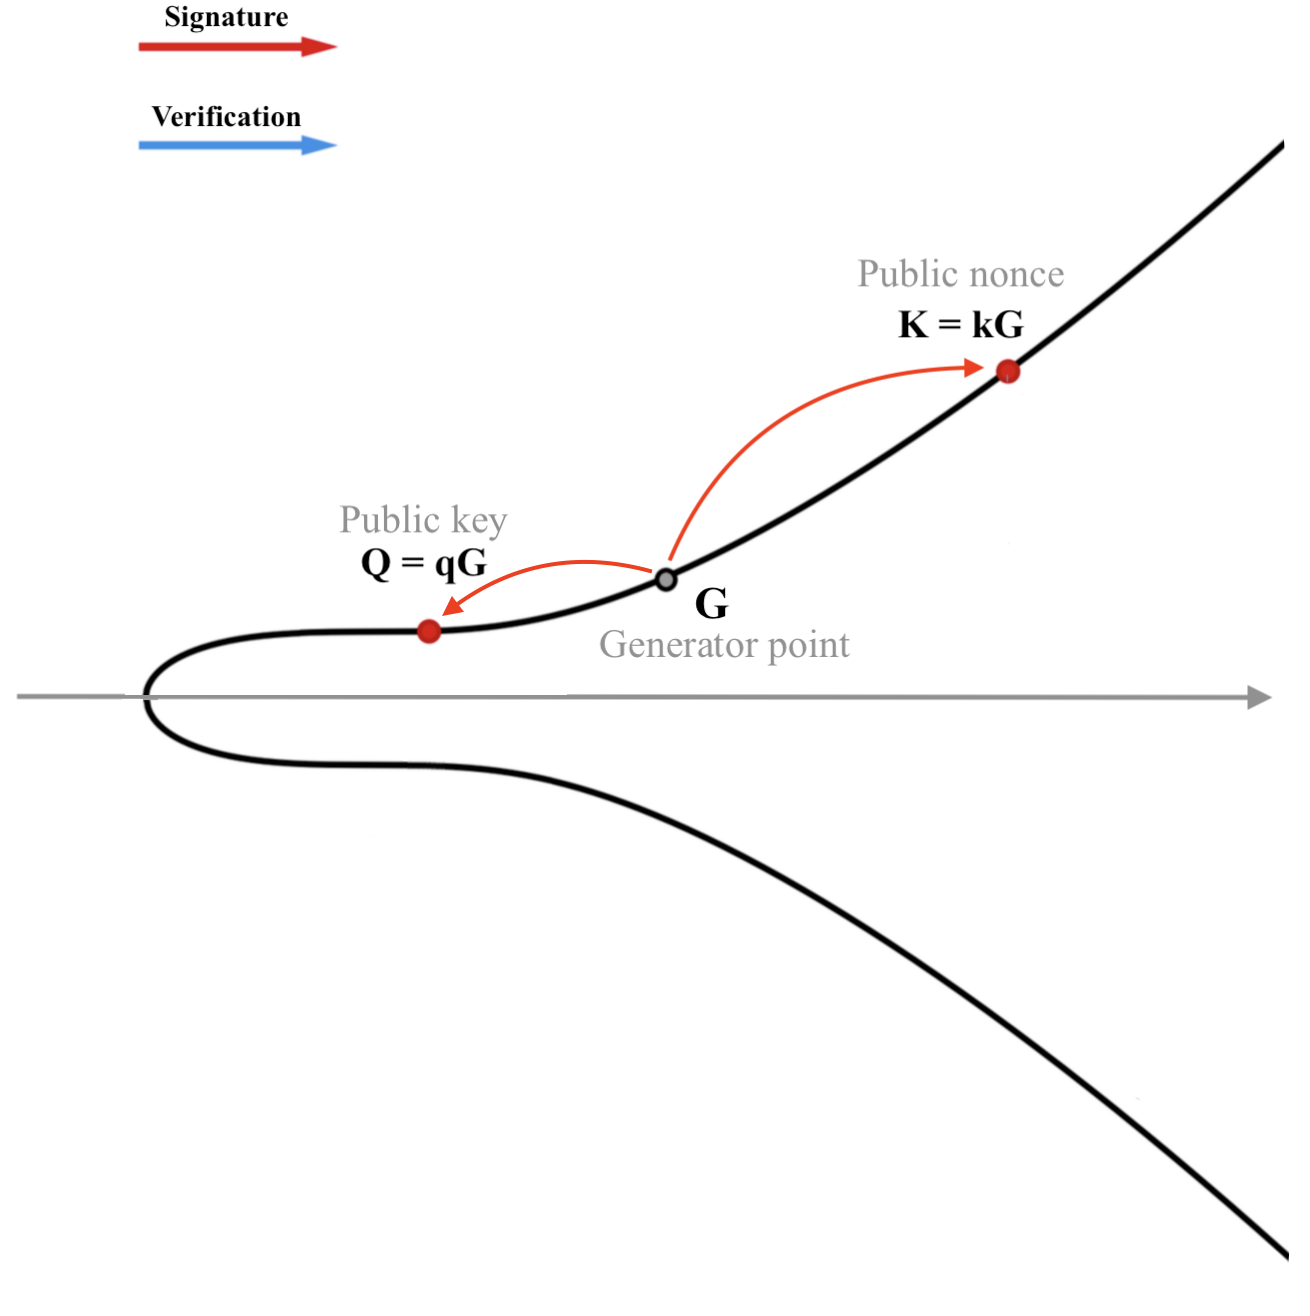
\includegraphics[scale=0.29]{Images/ECDSA3}
%				\source{\tiny \url{https://medium.com/cryptoadvance/how-schnorr-signatures-may-improve-bitcoin-91655bcb4744}}}
%				\only<5-8> {\vspace*{-0.5cm}
%					\hspace*{-1cm}
%					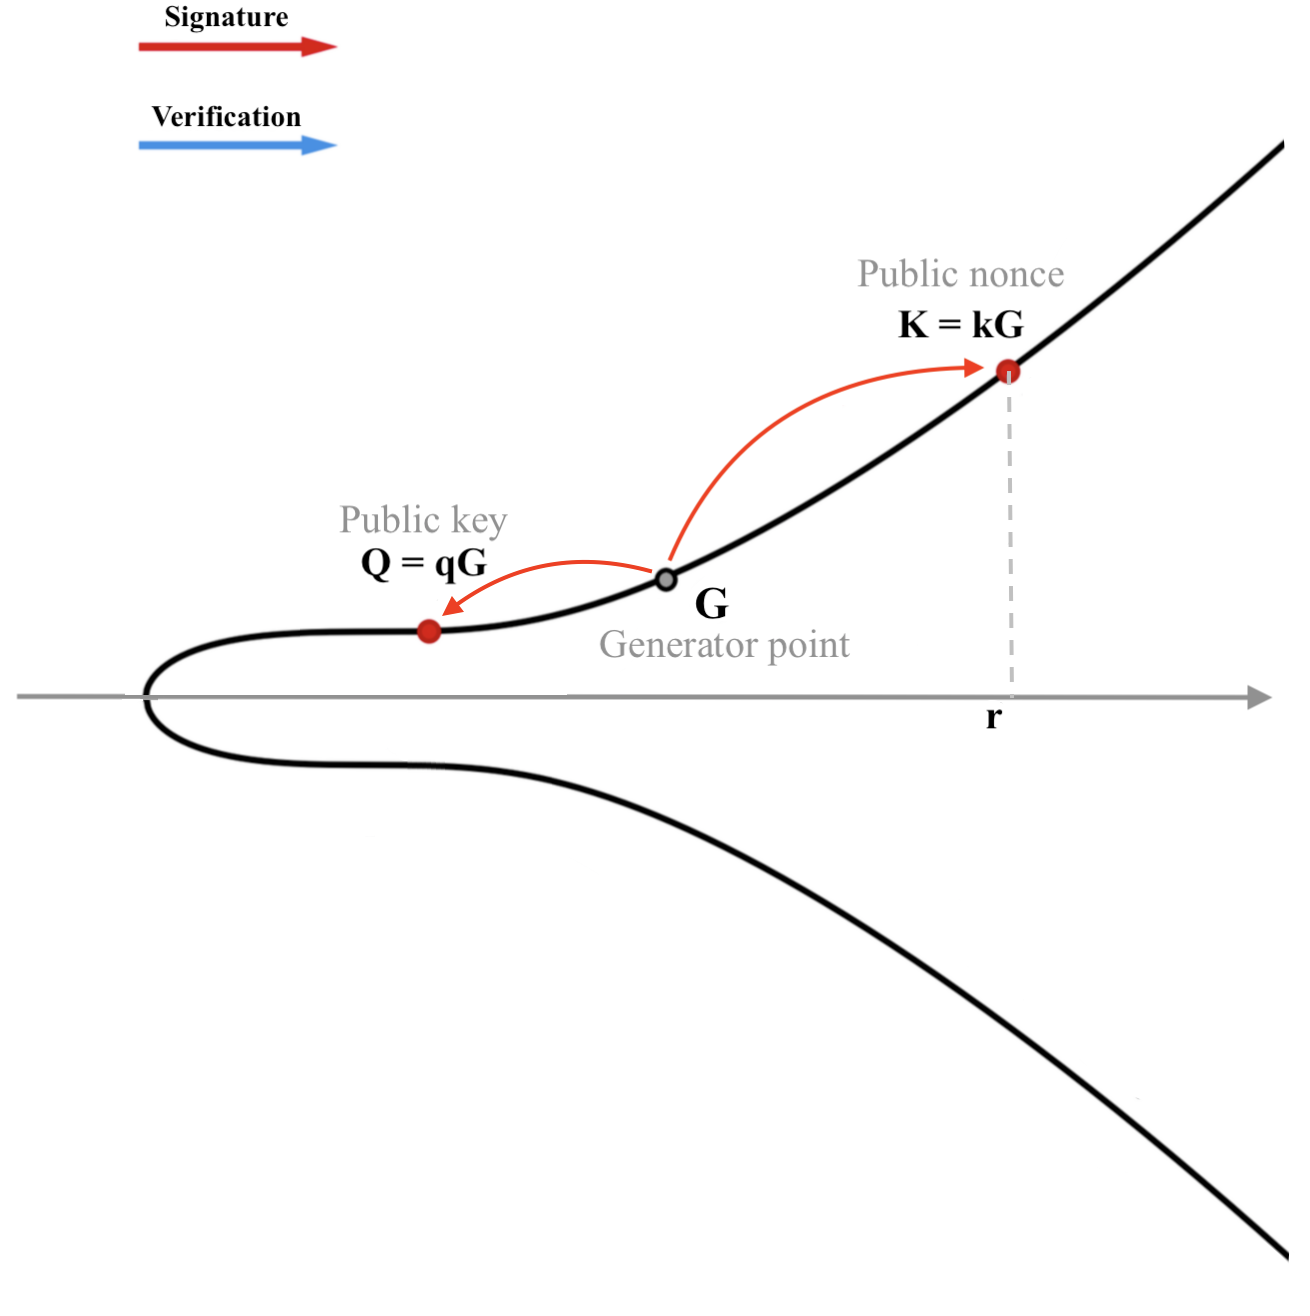
\includegraphics[scale=0.29]{Images/ECDSA4}
%				\source{\tiny \url{https://medium.com/cryptoadvance/how-schnorr-signatures-may-improve-bitcoin-91655bcb4744}}}
%				\end{figure}
%			\end{column}
%		\end{columns}
%	\end{frame}
%
%	\begin{frame}{Elliptic curve digital signature algorithm}
%		\begin{columns}
%			\begin{column}{0.6\linewidth}
%				ECDSA\_VER$((r,s), m, Q)$:
%				\begin{enumerate}
%					\item<2 -> \textbf{If} $r \notin \{1, ..., n - 1\}$ \textbf{or} $s \notin \{1, ..., n - 1\}$: \\ \textbf{\ \ \ return False};
%					\item<3 -> $e \gets \text{hash}(m)$;
%					\item<4 -> $u_1 \gets es^{-1} \ (\text{mod} \ n)$, $u_2 \gets rs^{-1} \ (\text{mod} \ n)$;
%					\item<5 -> $K \gets u_1G + u_2Q$;
%					\item<8 -> \textbf{return} $r = x_K \ (\text{mod} \ n)$.
%				\end{enumerate}
%			\end{column}
%			\begin{column}{0.5\linewidth}
%				\begin{figure}
%					\only<1-4> {\vspace*{-0.5cm}
%						\hspace*{-1cm}
%						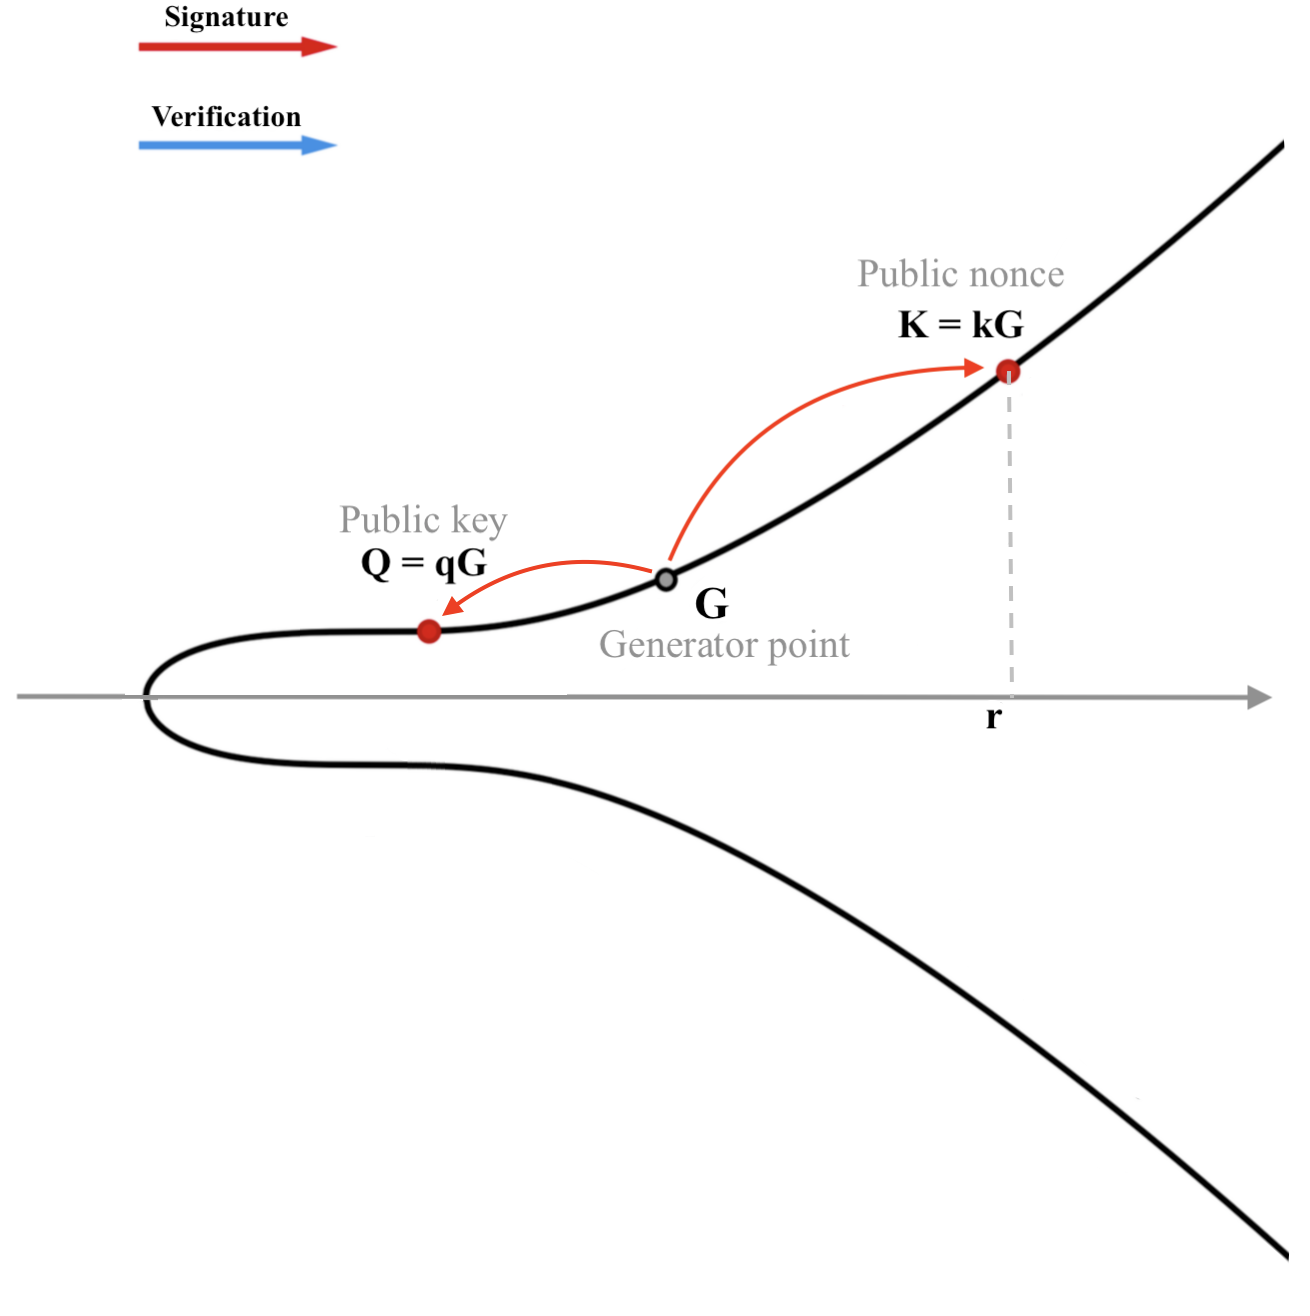
\includegraphics[scale=0.29]{Images/ECDSA4}
%						\source{\tiny \url{https://medium.com/cryptoadvance/how-schnorr-signatures-may-improve-bitcoin-91655bcb4744}}}
%					\only<5> {\vspace*{-0.5cm}
%						\hspace*{-1cm}
%						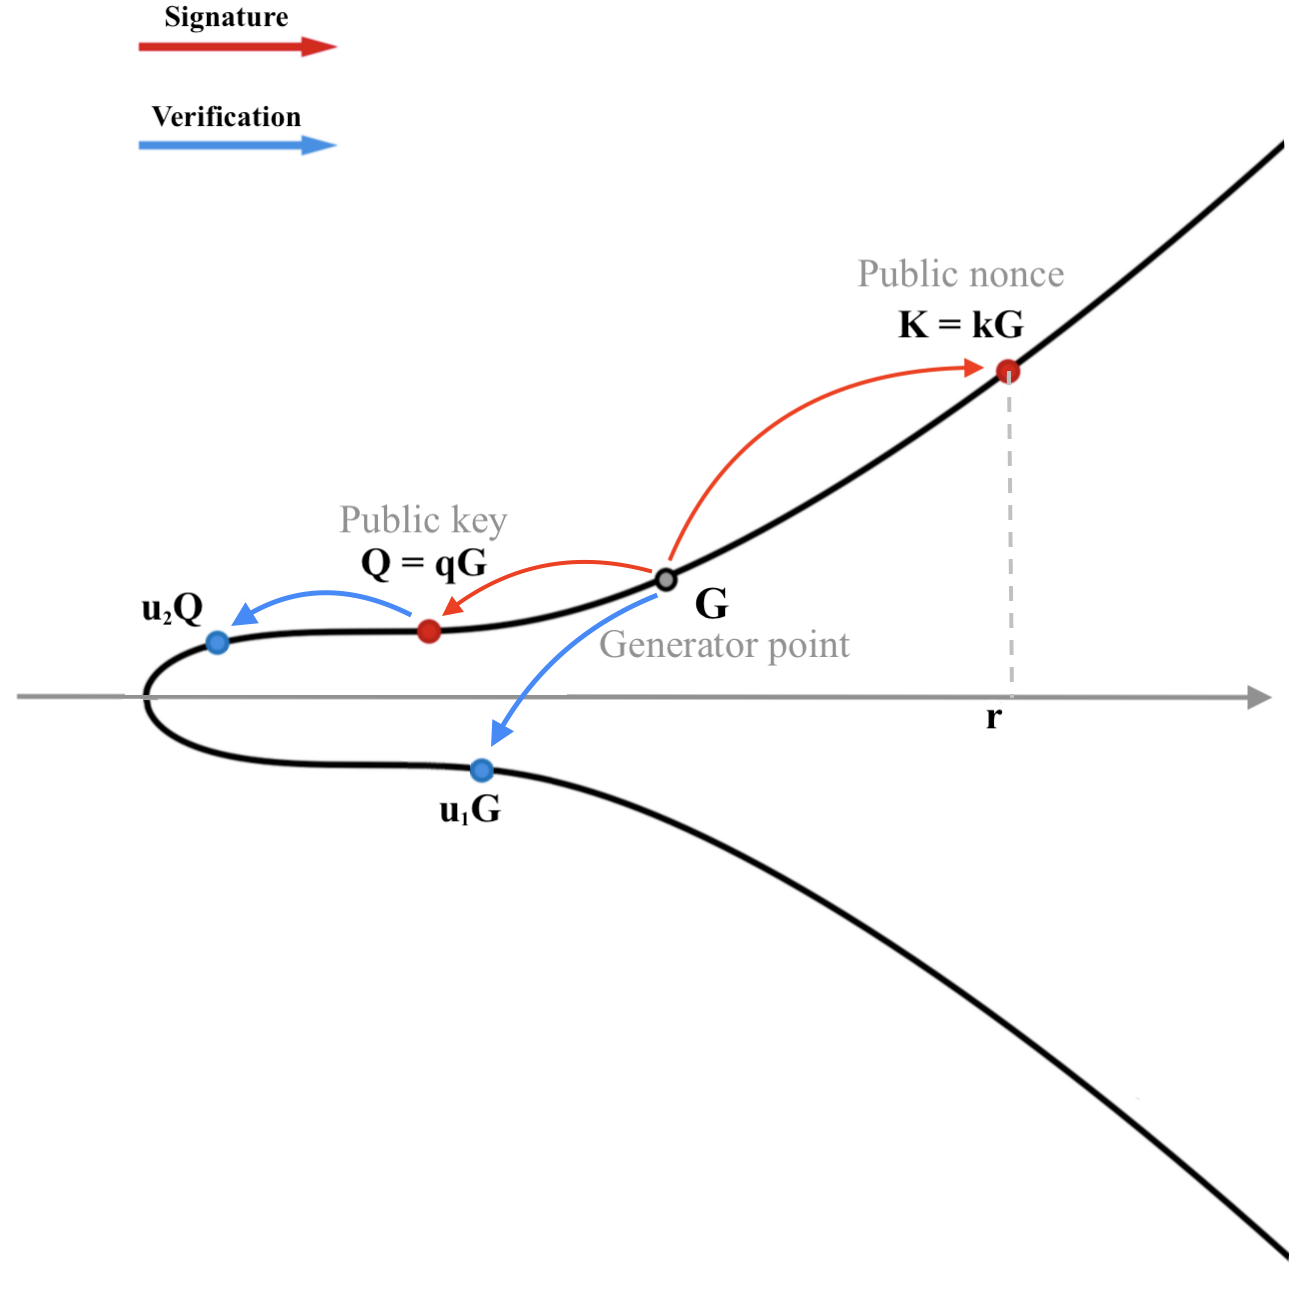
\includegraphics[scale=0.29]{Images/ECDSA5}
%						\source{\tiny \url{https://medium.com/cryptoadvance/how-schnorr-signatures-may-improve-bitcoin-91655bcb4744}}}
%					\only<6> {\vspace*{-0.5cm}
%						\hspace*{-1cm}
%						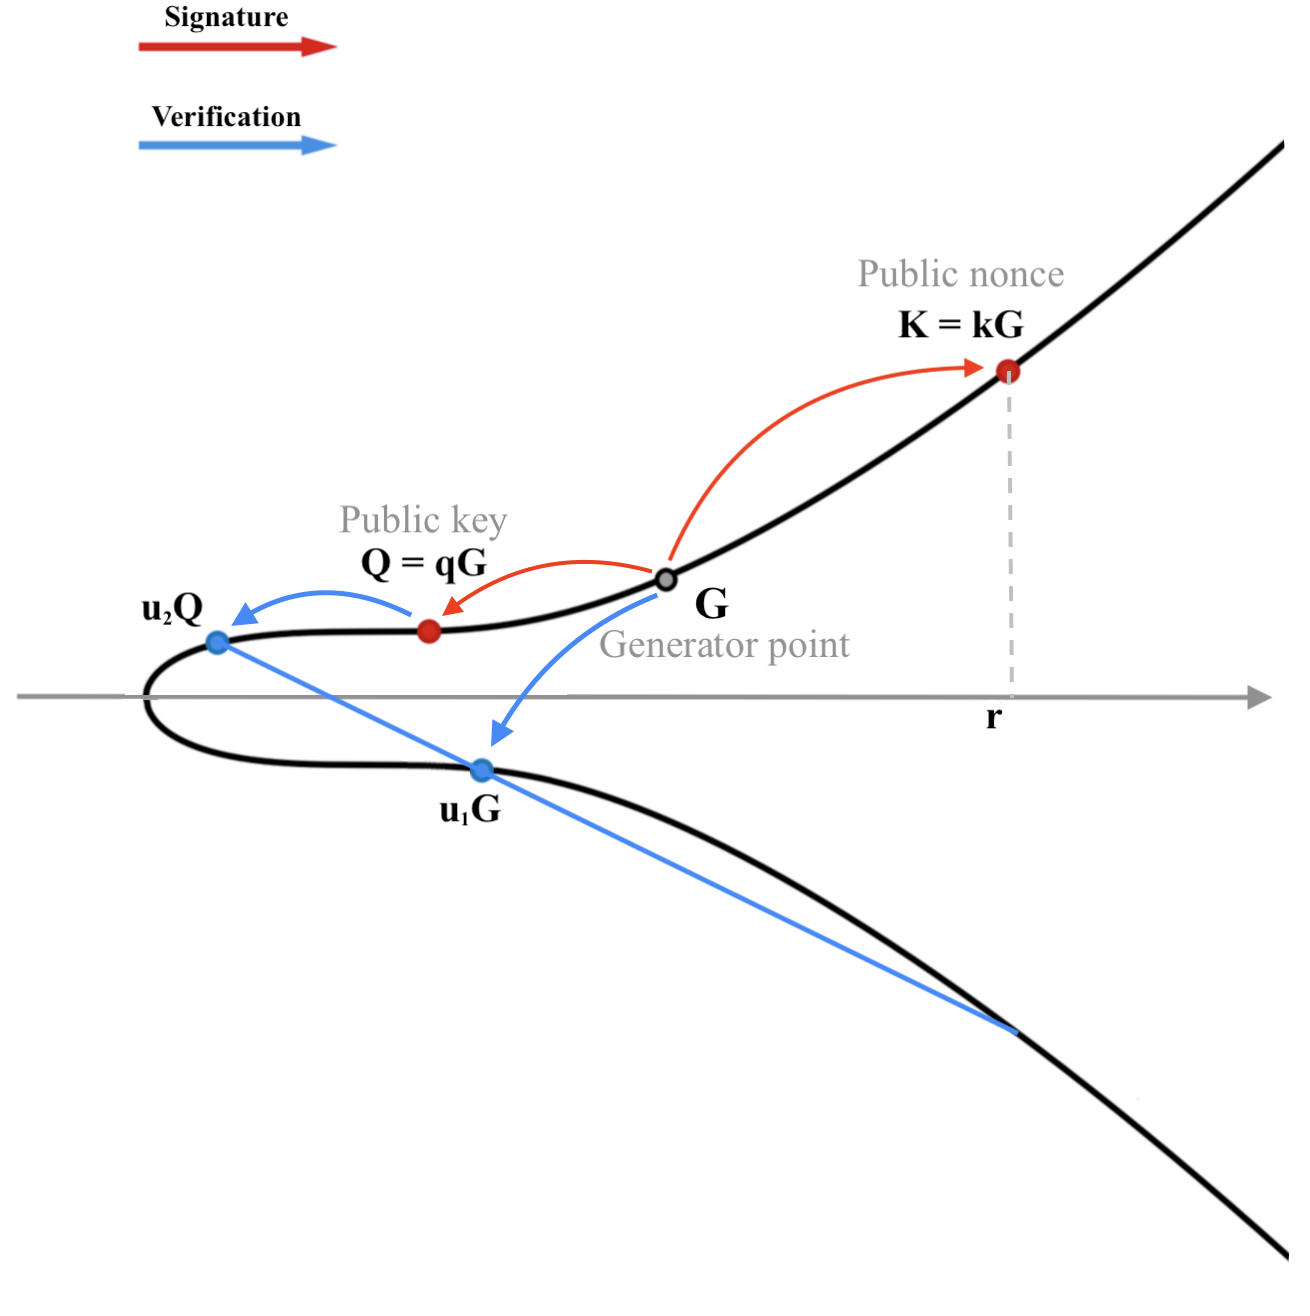
\includegraphics[scale=0.29]{Images/ECDSA6}
%						\source{\tiny \url{https://medium.com/cryptoadvance/how-schnorr-signatures-may-improve-bitcoin-91655bcb4744}}}
%					\only<7-8> {\vspace*{-0.5cm}
%						\hspace*{-1cm}
%						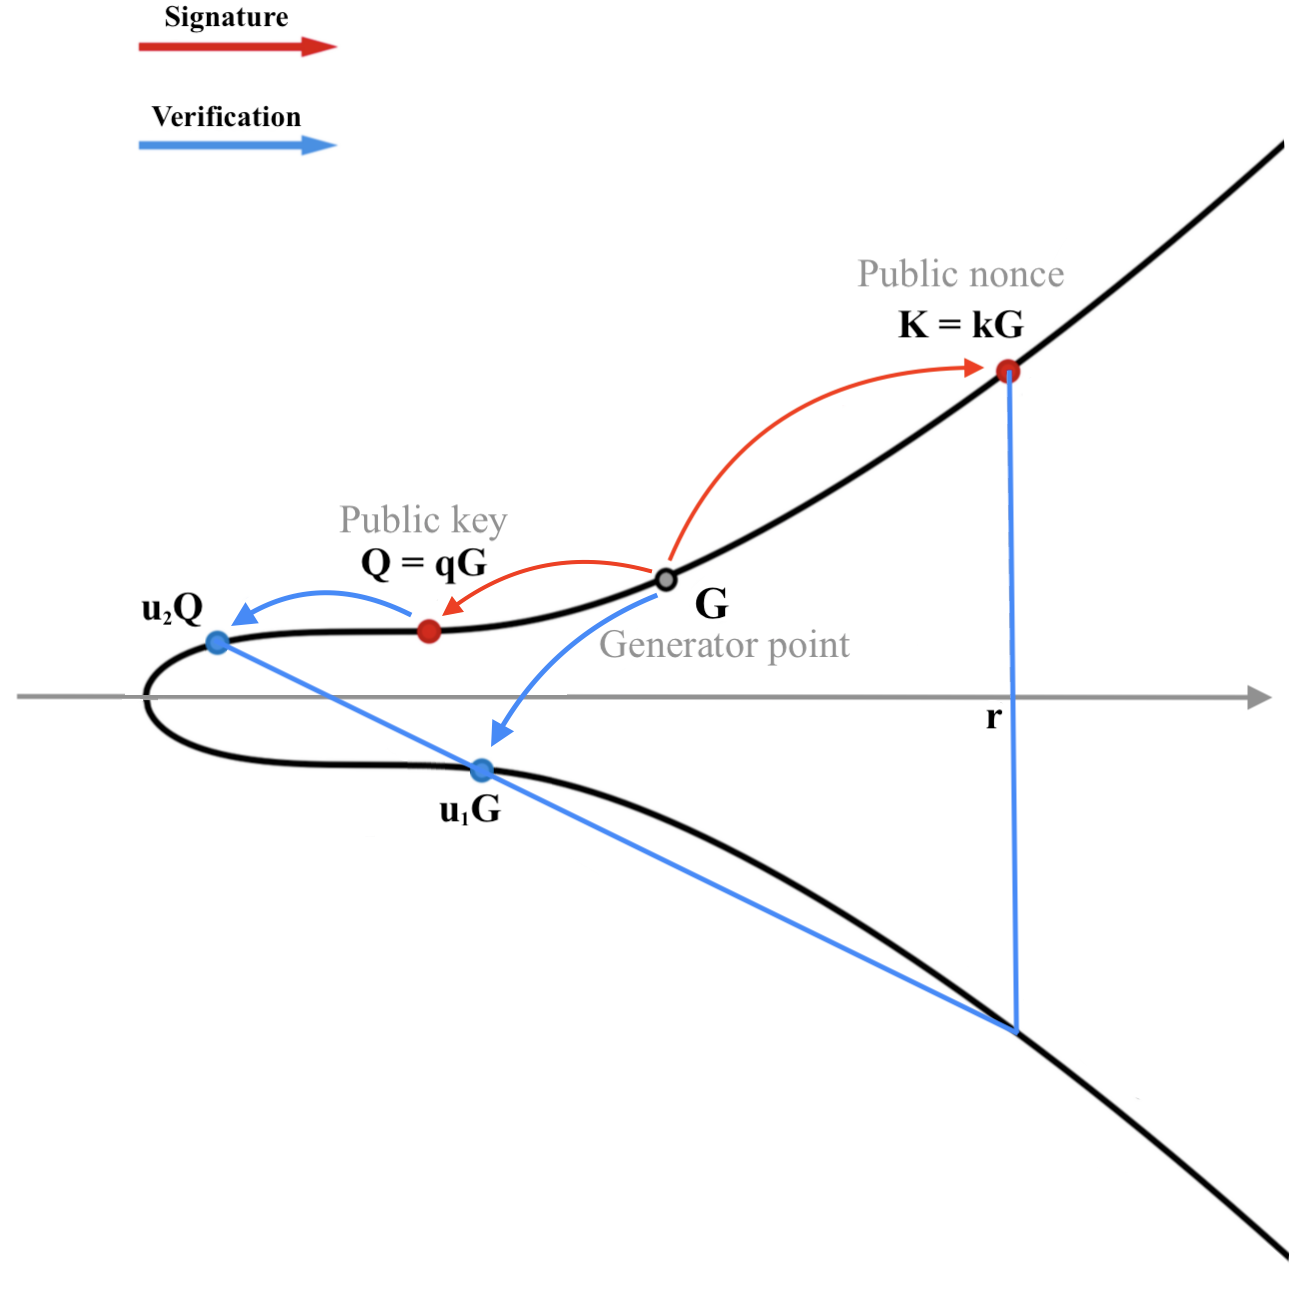
\includegraphics[scale=0.29]{Images/ECDSA7}
%						\source{\tiny \url{https://medium.com/cryptoadvance/how-schnorr-signatures-may-improve-bitcoin-91655bcb4744}}}
%				\end{figure}
%			\end{column}
%		\end{columns}
%	\end{frame}
%	
%	\subsection{ECSSA}
%	\begin{frame}{Elliptic curve Schnorr signature algorithm}
%		\begin{columns}
%			\begin{column}{0.6\linewidth}
%				\only<1>{ECDSA\_SIG$(m, q)$:}\only<2->{ECSSA\_SIG$(m, q)$:}
%				\begin{enumerate}
%					\item $k \xleftarrow{\text{\$}} \{1, ..., n - 1\}$;
%					\item $K \gets kG$;
%					\item \only<1>{$r \gets x_K \ (\text{mod} \ n)$;} \only<2->{\textcolor{red}{\textbf{If} $\text{jacobi}(y_K) \neq 1$: $k \gets n - k$;}}
%					\item \only<1-2>{$e \gets \text{hash}(m)$;} \only<3->{\textcolor{red}{$e \gets \text{hash}(x_K || qG || m) \ (\text{mod} \ n)$;}}
%					\item \only<1-3>{$s \gets k^{-1}(e + rq) \ (\text{mod} \ n)$;} \only<4->{\textcolor{red}{$s \gets k + eq \ (\text{mod} \ n)$;}}
%					\item \textbf{return} $(\only<1>{r}\only<2->{\textcolor{red}{x_K}}, s)$.
%				\end{enumerate}
%			\end{column}
%			\begin{column}{0.5\linewidth}
%				\begin{figure}
%					\only<1> {\vspace*{-0.5cm}
%						\hspace*{-1cm}
%						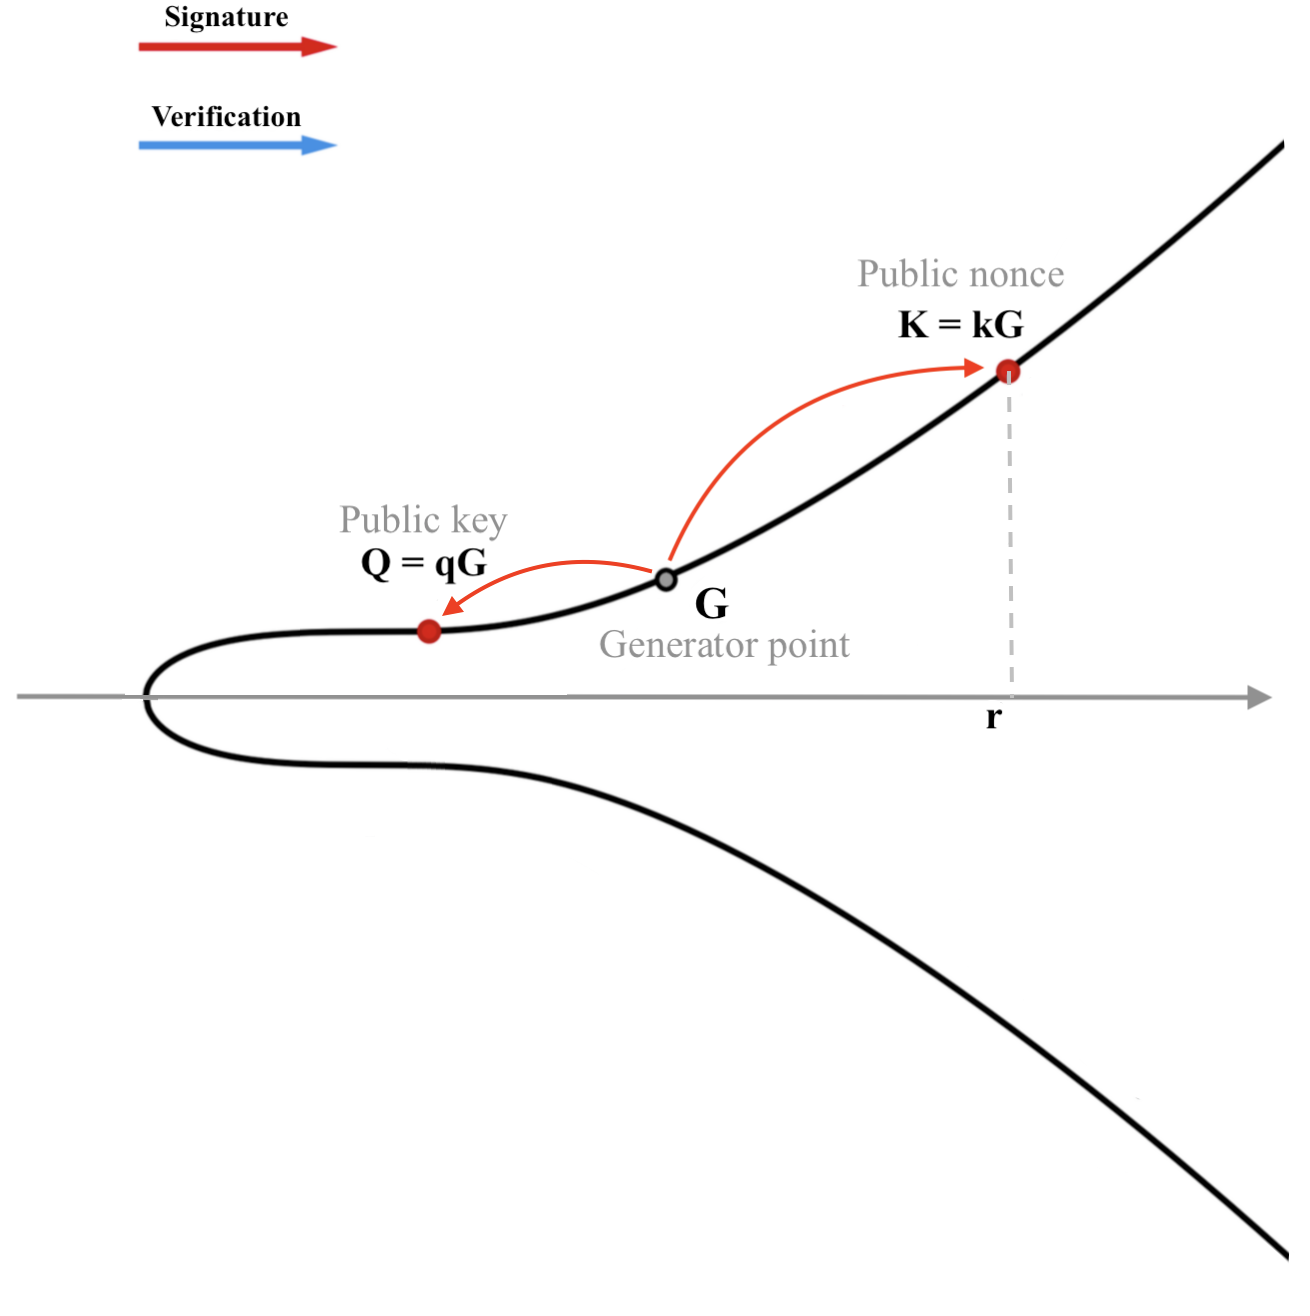
\includegraphics[scale=0.29]{Images/ECDSA4}
%						\source{\tiny \url{https://medium.com/cryptoadvance/how-schnorr-signatures-may-improve-bitcoin-91655bcb4744}}}
%					\only<2-> {\vspace*{-0.5cm}
%						\hspace*{-1cm}
%						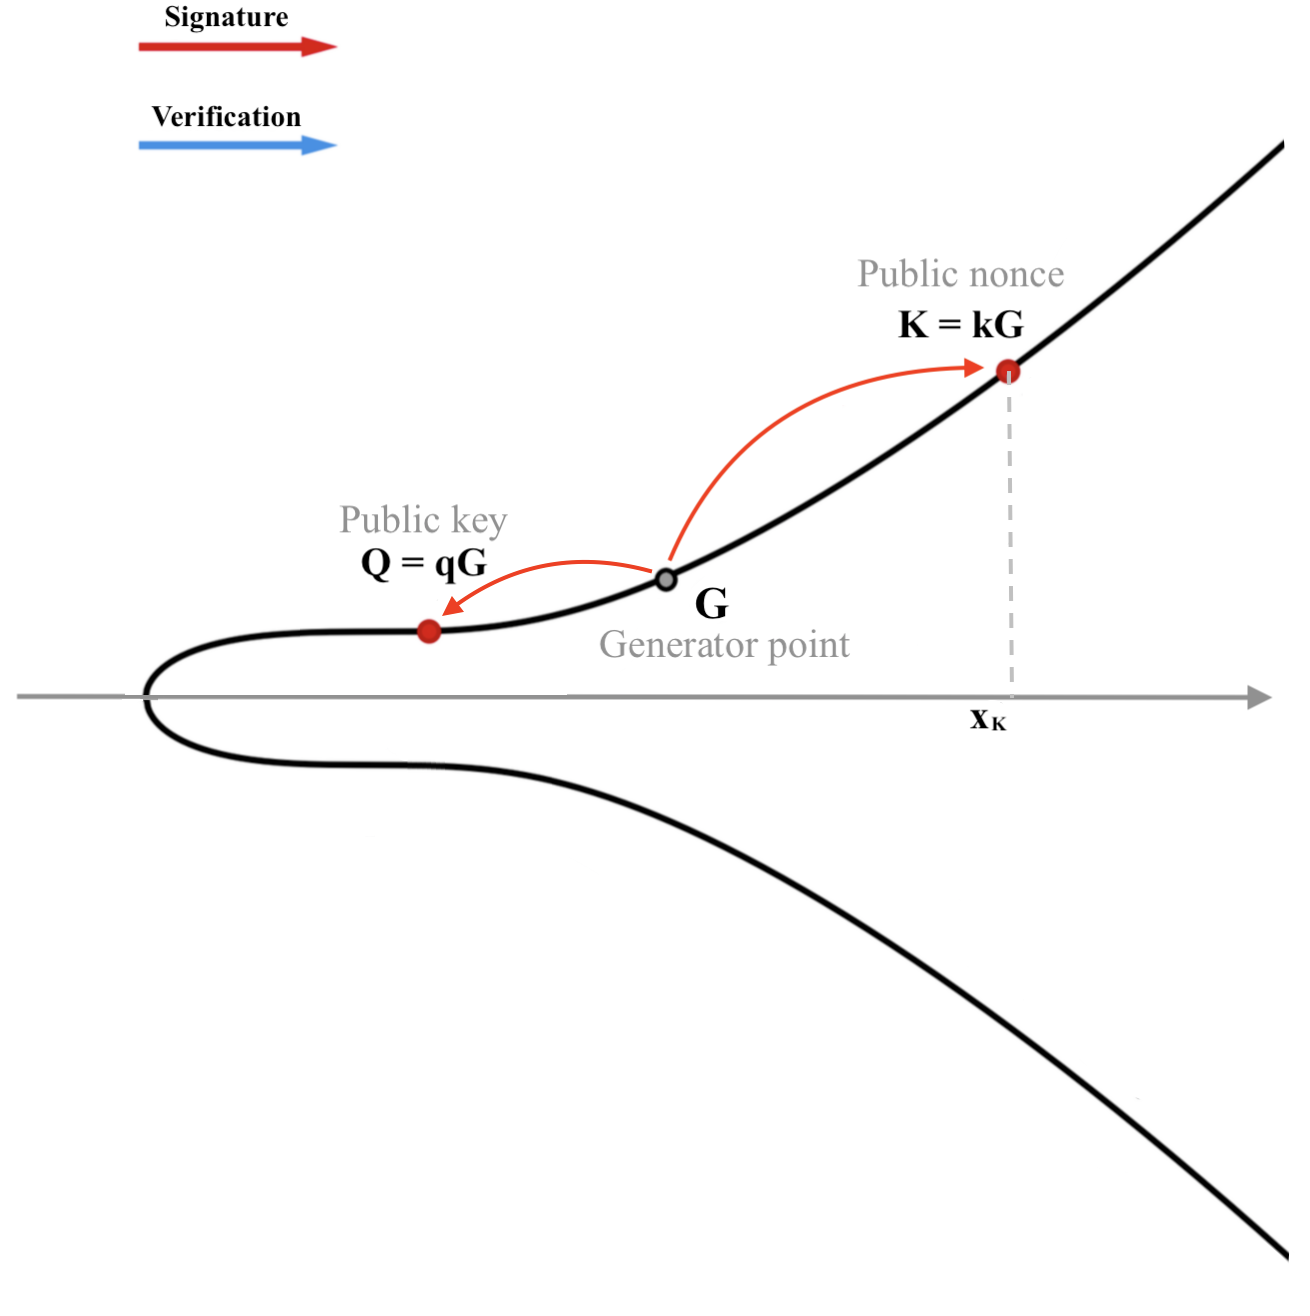
\includegraphics[scale=0.29]{Images/Schnorr1}
%						\source{\tiny \url{https://medium.com/cryptoadvance/how-schnorr-signatures-may-improve-bitcoin-91655bcb4744}}}
%				\end{figure}
%			\end{column}
%		\end{columns}
%	\end{frame}
%
%
%	\begin{frame}{Elliptic curve Schnorr signature algorithm}
%		\begin{columns}
%			\begin{column}{0.6\linewidth}
%				\only<1>{ECDSA\_VER$((r,s), m, Q)$:}\only<2->{ECSSA\_VER$((r, s), m, Q)$:}
%				\begin{enumerate}
%					\item \textbf{If} $r \notin \{1, ..., \only<1>{n}\only<2->{\textcolor{red}{p}} - 1\}$ \textbf{or} $s \notin \{1, ..., n - 1\}$: \\ \textbf{\ \ \ return False}; 
%					\item \only<1-2>{$e \gets \text{hash}(m)$;} \only<3->{\textcolor{red}{$e \gets \text{hash}(r || Q || m) \ (\text{mod} \ n)$;}}
%					\item \only<1-3>{$K \gets es^{-1}G + rs^{-1}Q$;} \only<4->{\textcolor{red}{$K \gets sG - eQ$;}}
%					\item \textbf{return} $r = x_K \only<1-4>{\ (\text{mod} \ n).}$ \only<1-4>{\\ \textcolor{white}{spazio necessario}} \only<5>{\textcolor{red}{\textbf{and} \\ $\ \ \ \ \ \ \text{jacobi}(y_K) = 1$.}}
%				\end{enumerate}
%			\end{column}
%			\begin{column}{0.5\linewidth}
%				\begin{figure}
%					\only<1-3> {\vspace*{-0.5cm}
%						\hspace*{-1cm}
%						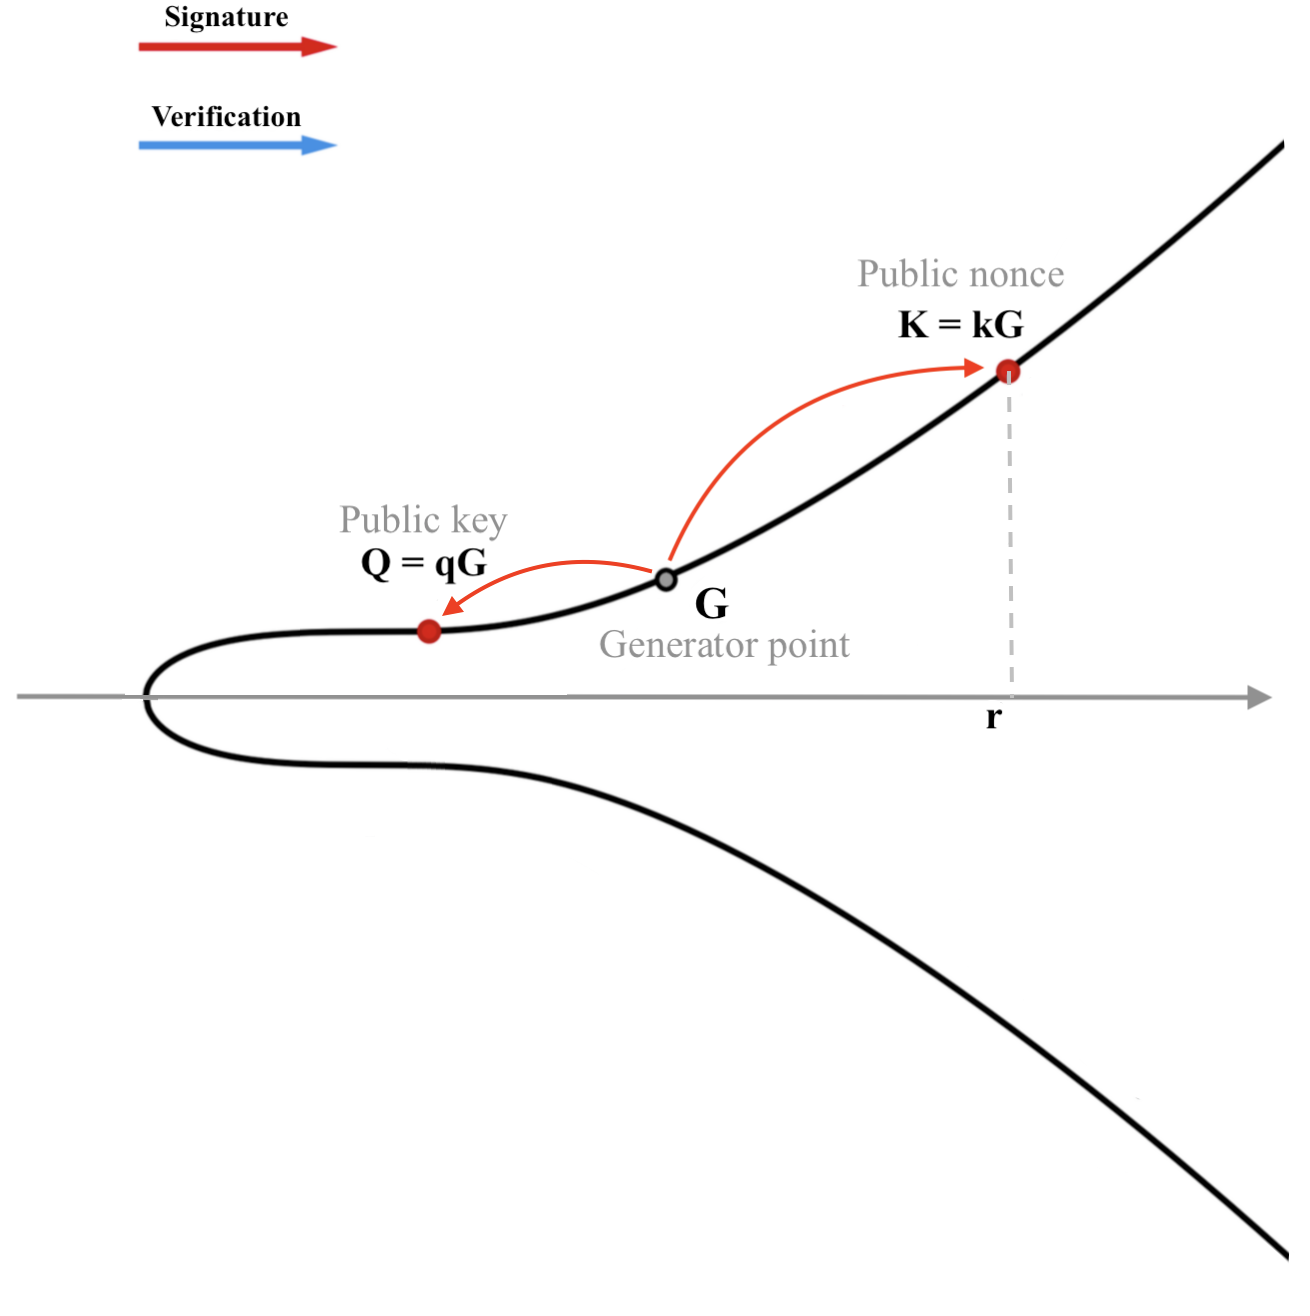
\includegraphics[scale=0.29]{Images/ECDSA4}
%						\source{\tiny \url{https://medium.com/cryptoadvance/how-schnorr-signatures-may-improve-bitcoin-91655bcb4744}}}
%					\only<4-> {\vspace*{-0.5cm}
%						\hspace*{-1cm}
%						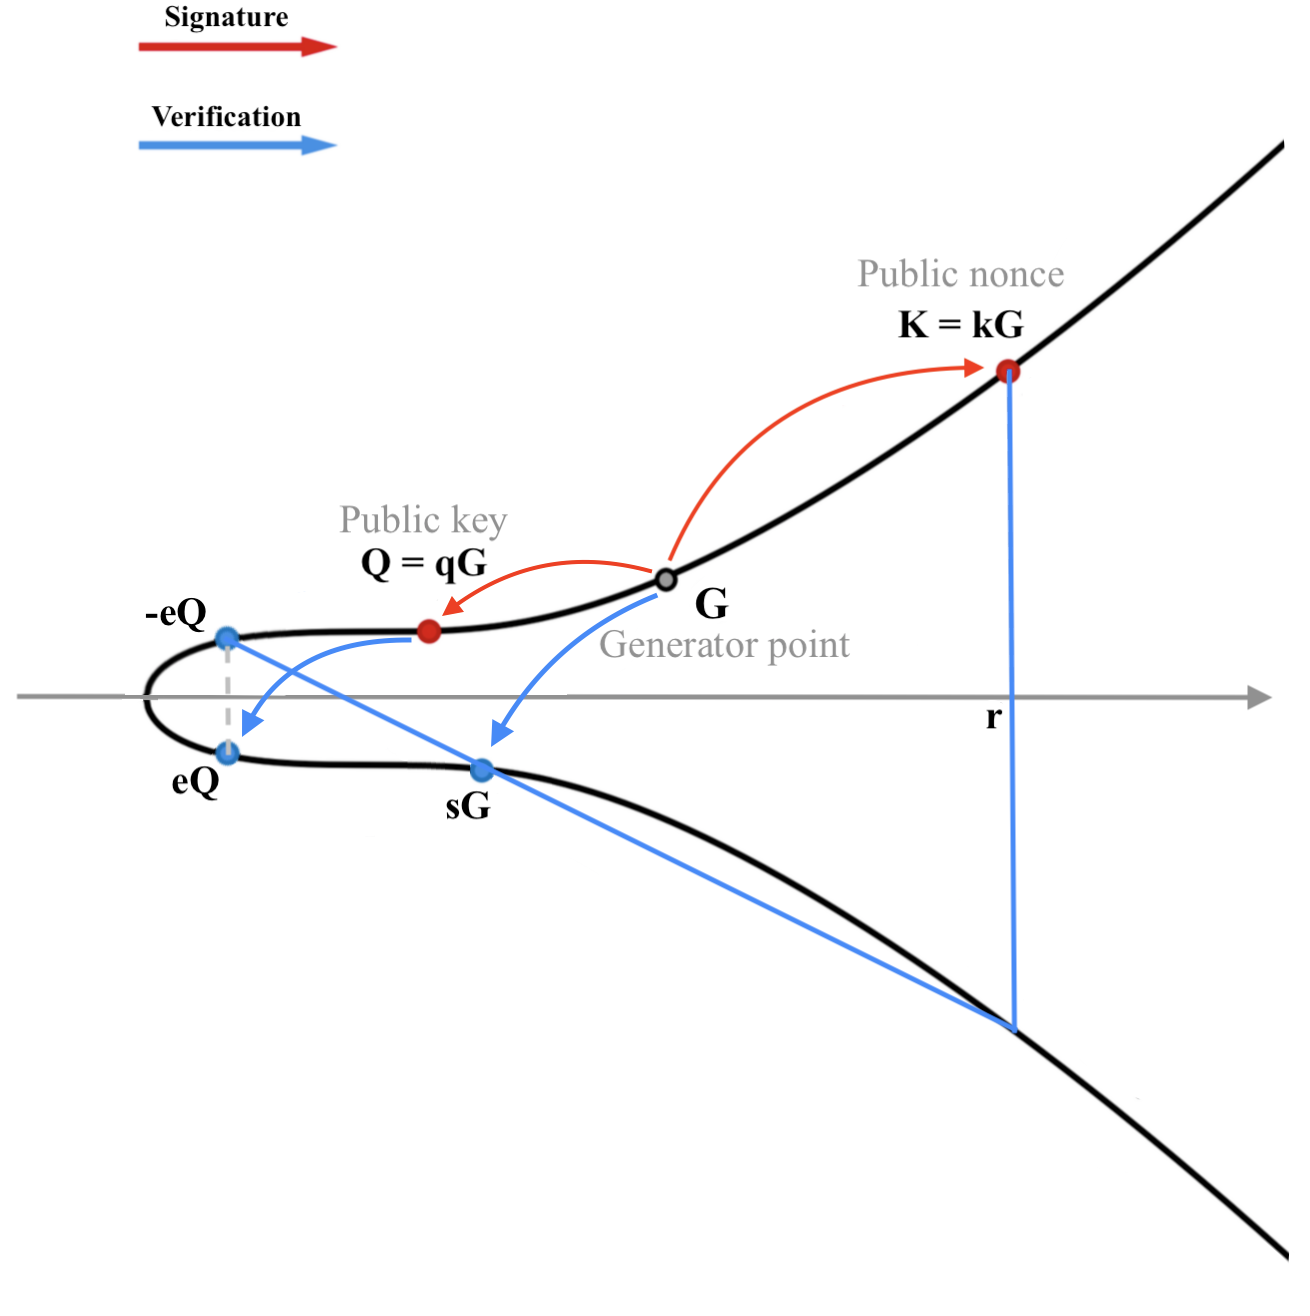
\includegraphics[scale=0.29]{Images/Schnorr6}
%						\source{\tiny \url{https://medium.com/cryptoadvance/how-schnorr-signatures-may-improve-bitcoin-91655bcb4744}}}
%				\end{figure}
%			\end{column}
%		\end{columns}
%	\end{frame}
%
%	\begin{frame}{ECDSA vs. ECSSA}
%		\begin{columns}
%			\begin{column}{0.5\linewidth}
%				ECDSA:
%				\begin{itemize}
%					\item<2 -> Malleable: given $(r, s)$ also $(r, -s \ (\text{mod} \ n))$ is a valid signature for same message and public key;
%					\item<3 -> DER encoding: variable length, up to 72 bytes;
%					\item<4 -> Chosen standardization forbid batch validation;
%					\item<5 -> Not linear: very complex higher level constructions.
%				\end{itemize}
%			\end{column}
%			\begin{column}{0.5\linewidth}
%				ECSSA:
%				\begin{itemize}
%					\item<2 -> Provably secure (SUF-CMA) in the Random Oracle Model assuming the ECDLP is hard $\Longrightarrow$ not malleable;
%					\item<3 -> New encoding: fixed length, always 64 bytes;
%					\item<4 -> \hyperlink{batch_validation}{Batch validation} scales logarithmically;
%					\item<5 -> Linear: easier higher level constructions.
%				\end{itemize}
%			\end{column}
%		\end{columns}
%	\end{frame}
%	
%	\section{ECSSA applications}
%	
%	\subsection{Bitcoin's smart contracts}
%	\begin{frame}{Bitcoin's smart contracts}
%		Bitcoin has been conceived as programmable money: the funds are locked by a smart contract that embeds the spending conditions.
%		
%		\bigskip
%		\noindent
%		In conjunction with signatures, they enforce the property right in the digital realm: this is why signatures are typically necessary to spend bitcoins and are required by the unlocking sripts.
%		
%		\bigskip
%		\noindent
%		\begin{block}{An easy example: Pay-to-Public-Key (P2PK)}
%			\begin{itemize}
%				\item Locking script: $<$pubKey$>$ OP\_CHECKSIG
%				\item Unlocking script: $<$sig$>$
%			\end{itemize}
%		\end{block}
%	\end{frame}
%	
%	\subsection{MuSig}
%	\begin{frame}{Multi-signature schemes}
%		Multi-signature schemes allow a group of users to cooperate to sign a single message: they are fundamental in real life applications.
%
%		\begin{block}{ECDSA multi-signature ($t$-of-$m$)}
%			\begin{itemize}
%				\item Locking script: t $<$pubKey1$>$ $<$pubKey2$>$ ... $<$pubKeym$>$ \hphantom{em} \hphantom{em} \hphantom{em} \hphantom{ipsem}m
%				OP\_CHECKMULTISIG
%				\item Unlocking script: 0 $<$sig1$>$ $<$sig2$>$ ... $<$sigt$>$
%			\end{itemize}
%		\end{block}
%	
%		\bigskip
%		\noindent
%
%		\onslide<2->{\alert<3>{Schnorr multi-signature (2-of-2) implemented naively:}
%		\begin{itemize}
%			\item\alert<3>{Alice ($\{q_A, Q_A\}$) and Bob ($\{q_B, Q_B\}$) generate $K_A$ and $K_B$;}
%			\item\alert<3>{They exchange them and set the public nonce at $K = K_A + K_B$. The joint public key is set at $Q = Q_A + Q_B$;}
%			\item\alert<3>{Their partial signatures are: $s_i = k_i + \text{hash}(x_K || Q || msg)q_i \ (\text{mod} \ n), \ i \in \{A, B\}$;}
%			\item\alert<3>{The signature $(x_K, s_A + s_B \ (\text{mod} \ n))$ is valid for $msg$ and $Q$.}
%		\end{itemize}}
%		\onslide<3>{\huge \centering \textcolor{red}{INSECURE: rogue key attack!}}
%	\end{frame}
%
%	\begin{frame}{\hyperlink{musig}{MuSig}: compact $m$-of-$m$ signature scheme}
%		To solve the problem without resorting to the Knowledge Of Secret Key (KOSK) assumption, the idea is to introduce a ``random factor" (ROM) $a_i = \text{hash}(\{Q_1,...,Q_m\} || Q_i)$ per public key $Q_i$:
%		$$Q = \onslide<2->{a_1}Q_1 + \onslide<2->{a_2}Q_2 + ... + \onslide<2->{a_m}Q_m.$$
%		\onslide<3->{
%		$$s_i = k_i + \text{hash}(x_K || Q || msg)a_iq_i \ (\text{mod} \ n), \ i = 1, ..., m.$$
%		The signature $(x_K,  s =  \sum_{i = 1}^{m}s_i \ (\text{mod} \ n))$ can be verified as a simple Schnorr signature against $Q$:
%		$$sG = \left(\sum_{i = 1}^{m}k_i + \text{hash}(x_K || Q || msg)\sum_{i = 1}^{m}a_iq_i\right)G  =$$
%		$$= \sum_{i = 1}^{m}K_i + \text{hash}(x_K || Q || msg)\sum_{i =  1}^{m}a_iQ_i =$$
%		$$= K + \text{hash}(x_K || Q || msg)Q.$$}
%	\end{frame}
%
%	\begin{frame}{\hyperlink{musig}{MuSig}: compact $m$-of-$m$ signature scheme}
%		\begin{itemize}
%			\item Compact: same size as the single user case;
%			\item Secure in the plain public key model: allows signature aggregation at transaction level;
%			\item Interactive: affects usability, prevents signature aggregation at block level;
%			\item Key aggregation: signature indistinguishable from the single user case.
%		\end{itemize}
%		The multi-signature policy is completely hidden: this is a huge improvement for both privacy and efficiency.
%	\end{frame}
%	
%
%	\subsection{Threshold signature scheme}
%	\begin{frame}{\hyperlink{threshold}{Threshold signature scheme} ($t$-of-$m$)}
%		\begin{itemize}
%			\item Pedersen verifiable secret sharing scheme:
%			\begin{itemize}
%				\item A dealer chooses secret $r \in \{1, ..., n - 1\}$;
%				\item He embeds it in a random polynomial of degree $t - 1$:
%				$f(u) = r + f_1u + ... + f_{t - 1}u^{t - 1} \ (\text{mod} \ n)$, $f_1, ..., f_{t - 1}\xleftarrow{\text{\$}} \{0, ..., n - 1\}$;
%				\item Each participant $i = 1, ..., m$ of the scheme receives the share $s_i = f(i)$;
%				\item The secret is reconstructed by any coalition $\mathcal{P}$ with $|\mathcal{P}| = t$ via Lagrange's interpolation formula: $r = f(0) = \sum_{i \in \mathcal{P}}s_i\prod_{h \in \mathcal{P}, h \neq i}\frac{h}{h - i} \ (\text{mod} \ n)$.
%			\end{itemize}
%			\onslide<2->{
%			\item Protocol for the generation of a shared random secret: every participant acts as the dealer in the previous protocol with secret $r_i$ and sharing polynomial $f_i(u)$:
%			\begin{itemize}
%				\item Shared secret: $r = \sum_{i = 1}^{m}r_i \ (\text{mod} \ n) \ \Longrightarrow \ \{r, R\}$;
%				\item Global sharing polynomial: $F(u) = \sum_{i = 1}^{m}f_i(u) \ (\text{mod} \ n)$;
%				\item Share of the secret belonging to $i$: $s_i = \sum_{j = 1}^{m}f_j(i) \ (\text{mod} \ n) = F(i)$.
%			\end{itemize}}
%		\end{itemize}
%	\end{frame}
%
%	\begin{frame}{\hyperlink{threshold}{Threshold signature scheme} ($t$-of-$m$)}
%		\begin{itemize}
%			\item The protocol for the generation of a shared random secret is run twice to establish a key pair $\{q, Q\}$ (shares $\alpha_i = F_1(i)$, $i = 1, ..., m$) and a nonce pair $\{k, K\}$ (shares $\beta_i = F_2(i)$, $i = 1, ..., t$);
%			\item Each signer $i = 1, ..., t$ computes his partial signature as: $\gamma_i = \beta_i + e\alpha_i \ (\text{mod} \ n)$, $e = \text{hash}(x_K || Q || msg) \ (\text{mod} \ n)$;
%			\item The signature is $(x_K, s)$, with $s = \sum_{i = 1}^{t}\gamma_i\prod_{h \neq i}\frac{h}{h - i} \ (\text{mod} \ n)$.
%		\end{itemize}
%		
%		$s$ computed in this way satisfies $s = k + eq \ (\text{mod} \ n)$: 
%		$$F_3(u) := F_2(u) + eF_1(u) \ \Longrightarrow$$ 
%		$$\Longrightarrow \ s := F_3(0) = F_2(0) + eF_1(0) = k + eq \ (\text{mod} \ n).$$
%		$$F_3(i) = F_2(i) + eF_1(i) = \beta_i + e\alpha_i \ (\text{mod} \ n) = \gamma_i.$$
%	\end{frame}
%
%	\begin{frame}{ECDSA vs. ECSSA (multi-signature)}
%		\begin{block}{ECDSA}
%			\begin{itemize}
%				\item Locking script: t $<$pubKey1$>$ $<$pubKey2$>$ ... $<$pubKeym$>$ \hphantom{em} \hphantom{em} \hphantom{em} \hphantom{ipsem}m
%				OP\_CHECKMULTISIG
%				\item Unlocking script: 0 $<$sig1$>$ $<$sig2$>$ ... $<$sigt$>$
%			\end{itemize}
%		\end{block}
%	
%		$\Longrightarrow$ 33 bytes * $m$ + 70 bytes * $t$. 
%		
%		\bigskip
%		\noindent
%		\begin{block}{ECSSA}
%			\begin{itemize}
%				\item Locking script: $<$jointPubKey$>$ OP\_SCHNORR
%				\item Unlocking script: $<$jointSig$>$
%			\end{itemize}
%		\end{block}
%	
%	 $\Longrightarrow$ 33 bytes + 64 bytes.
%	\end{frame}
%
%
%	\section{Conclusion}
%	\begin{frame}{Conclusion}
%		We have seen that Schnorr would result in huge privacy (fungibility) and efficiency (scalability) improvements for Bitcoin:
%		\begin{itemize}
%			\item  Batch validation: a group of signatures could be validated much faster;
%			\item Smaller key size, aggregation at transaction level, and hidden policies;
%			\item Improved security, being Schnorr provably secure.
%		\end{itemize}
%	
%	\onslide<2->{But there is even more:
%		\begin{itemize}
%			\item \hyperlink{adaptor}{Adaptor signatures}: they aim at reducing the verbose scripting semantics to a fixed size signature with huge benefits for privacy and efficiency in protocols like atomic swaps and the Lightning Network;
%			\item Taproot: built on top of the concepts of Merkelized Abstract Syntax Tree (MAST) and Pay-To-Contract, its aim is to make any arbitrary script to look the same as a single signer transaction in the cooperative case.
%		\end{itemize}}
%	\end{frame}
%	
%	\begin{frame}[t, allowframebreaks]
%	\frametitle{References}
%    	\setbeamertemplate{bibliography item}[text]
%    	\bibliographystyle{plain}
%		\nocite{*}
%		\bibliography{biblio}
%	\end{frame}
%	
%	\appendix
%	\backupbegin
%	\begin{frame}[label=point_addition]{Point addition - Geometric interpretation}
%		\begin{columns}
%			\begin{column}{0.5\linewidth}
%				The intuition to add points belonging to an EC defined over a finite field is the same presented for the curve defined over the real numbers: draw the line passing through the points (that repeats along the plane in this case) until it intersects a third point: then reflect this point with respect to the line $y = \frac{p}{2}$, i.e. apply the transformation $(x_3, y_3) \to (x_3, p - y_3)$.
%			\end{column}
%			\begin{column}{0.6\linewidth}
%				\begin{tikzpicture}[
%				every node/.style = {% is not necessary, default node's shape is rectangle
%					align=center}
%				]
%				
%				\node () at (0,0) {};
%				\node (a) {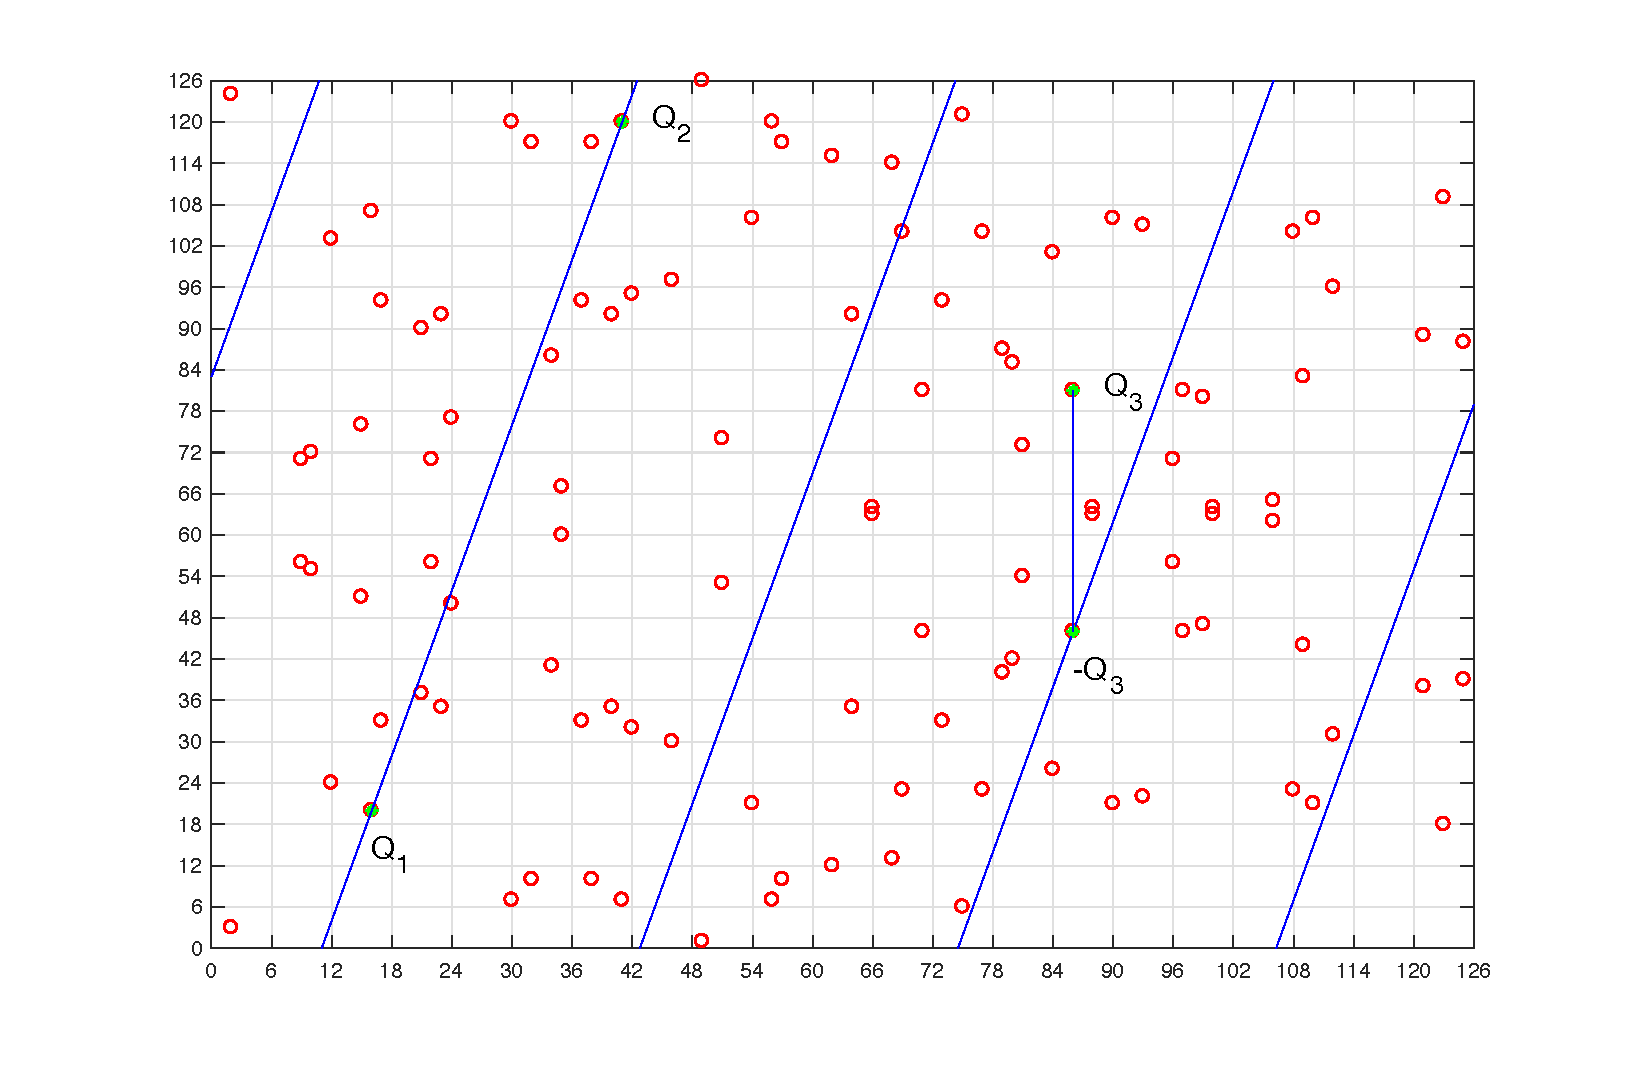
\includegraphics[height=5cm, width=6.6cm]{Images/sum_ec_over_ff}};
%				
%				\node (b) [below=of a, yshift = 1.2cm] {\small The curve $y^2 = x^3 - x + 3 \ \text{over} \ \mathbb{F}_{127}$.};
%				\end{tikzpicture}
%			\end{column}
%		\end{columns}
%	\end{frame}
%
%	\begin{frame}{Point addition - Algebraic formulas}
%		There are some cases to be considered:
%		\begin{itemize}
%			\item $Q_2 = -Q_1$: by definition we have $Q_1 + Q_2 = \infty$, where $\infty$ is the identity element of the addition operation;
%			\item $Q_2 = \infty$: $Q_1 + Q_2 = Q_1$;
%			\item $Q_2 = Q_1$: $x_3 = m^2 - 2x_1$ and $y_3 = m(x_1 - x_3) - y_1$, where $m = \frac{3x_1^2 + a}{2y_1}$;
%			\item $Q_2 \neq \pm Q_1$: $x_3 = m^2 - x_1 - x_2$ and $y_3 = m(x_1 - x_3) - y_1$, where $m = \frac{y_2 - y_1}{x_2 - x_1}$.
%		\end{itemize}
%	\end{frame}
%	
%	\begin{frame}[label = double_add]{Double and add algorithm}
%		Scalar multiplication is the core of ECC due to its computational asymmetry:
%		\begin{itemize}
%			\item The direct operation $q \mapsto Q$ can be made efficiently (i.e. there exist some polynomial time algorithms);
%			\item The inverse operation $Q \mapsto q$ in general cannot be made efficiently (i.e. do not exist sub-exponential algorithms).
%		\end{itemize}
%	
%		\bigskip
%		\noindent
%			
%		\begin{block}{Double and add algorithm: $q = 41$}
%			We decompose $q$ according to its binary representation:
%			$$41 = 1 + 8 + 32  \ \Longrightarrow \ 41G = G + 8G + 32G.$$
%			
%			\noindent
%			5 point doubling and 2 additions vs. 40 additions.
%	\end{block}
%	\end{frame}
%
%	\begin{frame}[label = batch_validation]{Batch validation}
%		A signature $(K, s)$ is valid if $K = sG - \text{hash}(x_K \ || \ Q \ || \ m)Q$. Thus, two valid signatures $(K_0, s_0)$ and $(K_1, s_1)$ satisfies:
%		$$K_0 + K_1 = (s_0 + s_1)G - \text{hash}(x_{K_0} \ || \ Q_0 \ || \ m_0)Q_0 - \text{hash}(x_{K_1} \ || \ Q_1 \ || \ m_1)Q_1.$$
%		Insecure (cancelation attack): introduction of random factors.
%		$$a_0K_0 + a_1K_1 =$$ $$
%		= (a_0s_0 + a_1s_1)G - a_0\text{hash}(x_{K_0} \ || \ Q_0 \ || \ m_0)Q_0 - a_1\text{hash}(x_{K_1} \ || \ Q_1 \ || \ m_1)Q_1.$$
%	\end{frame}
%
%	\begin{frame}{Batch validation - Bos-Coster's algorithm}
%		\begin{columns}
%			\begin{column}{0.5\linewidth}
%				$\ \ \ \ \ \ \ \ \ \ a_0K_0 + a_1K_1 =$ \\ $= (a_0 - a_1)K_0 + a_1(K_0 + K_1)$.
%				
%				\bigskip
%				
%				\begin{itemize}
%					\item Sort the tuples $(a_i, K_i)$ according to $a_i$ in descending order;
%					\item While the list has length larger than one:
%					\begin{itemize}
%						\item Substitute $(a_0, K_0)$ and $(a_1, K_1)$ with $(a_0 - a_1, K_0)$ and $(a_1, K_0 + K_1)$;
%						\item Sort the list again;
%					\end{itemize}
%					\item When only one element remains, with very large probability it will be of the form $(1, K)$, otherwise it will be of the form $(a, K)$.
%				\end{itemize}
%			\end{column}
%			\begin{column}{0.5\linewidth}
%				\hspace*{0cm}
%				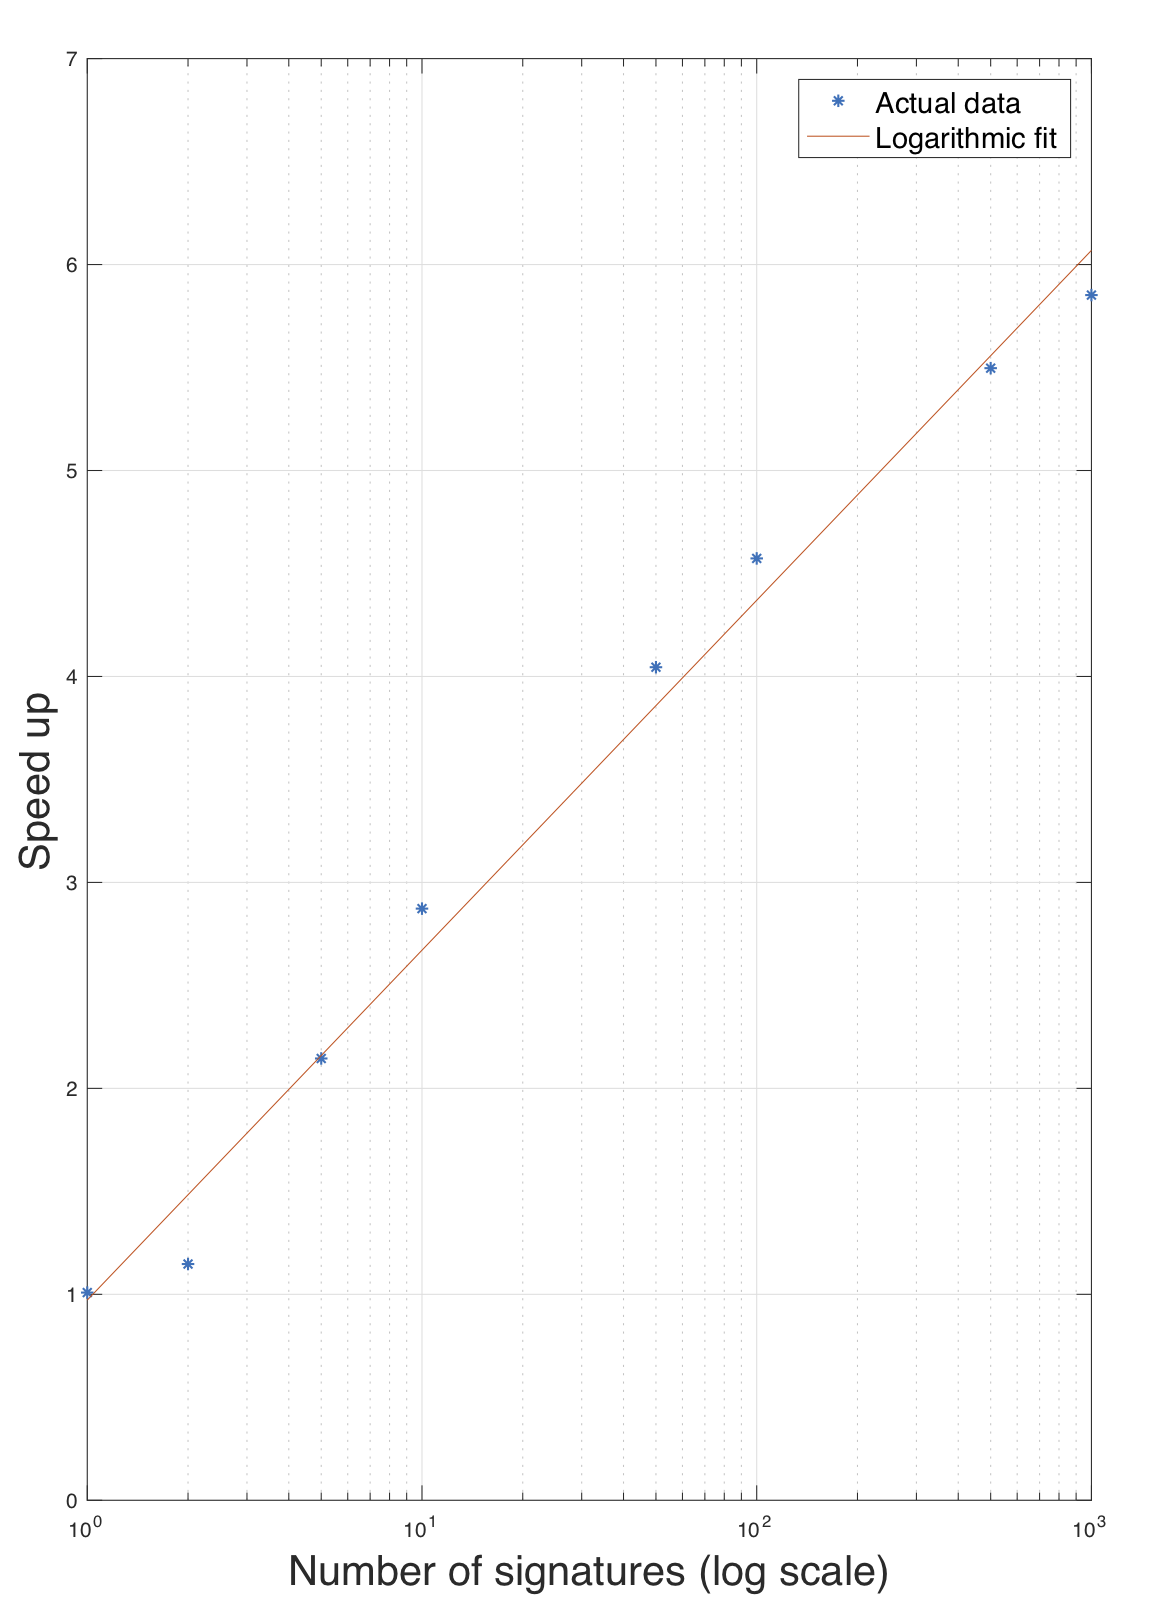
\includegraphics[scale=0.3]{Images/speedup}
%			\end{column}
%		\end{columns}
%	\end{frame}
%
%		\subsection{Adaptor signatures}
%		\begin{frame}[label = adaptor]{Adaptor signatures}
%		Building block for \textit{scriptless script}: aim at encapsulating the flexibility of script semantics in fixed size signatures.
%	
%		\bigskip
%		\noindent
%		The idea is to add to the public nonce $K$ a random $T = tG$ (public adaptor) but still consider $k$ 	as private nonce: this results in an invalid signature, however learning $t$ (private adaptor) is equivalent to learn a valid signature:
%		$$(x_T, x_{K + T}, \tilde{s}), \ \tilde{s} = k + \text{hash}(x_{K + T}||Q||m)q \ (\text{mod} \ n).$$
%		{\centering
%		Consistency equation: $\tilde{s}G = K + \text{hash}(x_{K + T}||Q||m)Q.$
%		\par}
%	
%		\bigskip
%		\noindent
%		Adaptor signatures can be used in conjunction with the MuSig protocol:
%		a signer generates $s_i' = k_i + \text{hash}(x_K || Q || msg)a_iq_i \ (\text{mod} \ n)$ after having used $K_i + T$ as public nonce.
%	\end{frame}
%
%	\begin{frame}{Cross-chain atomic swaps}
%		Exchange of different crypto-currencies among two distrustful users in an atomic and decentralized way.
%		\\
%		Nowadays, this is achieved via Hashed TimeLock Contract:
%		\begin{block}{HTLC}
%			\begin{itemize}
%				\item Locking script: \\
%				\ \ OP\_IF
%				\\
%				\ \ \ \ \ \ \ OP\_HASH256 $<$digest$>$ OP\_EQUALVERIFY OP\_DUP \\ 
%				\ \ \ \ \ \ \ OP\_HASH160 $<$Bob address$>$ \\
%				\ \ OP\_ELSE \\
%				\ \ \ \ \ \ \ $<$num$>$ OP\_CHECKSEQUENCEVERIFY OP\_DROP \\ 
%				\ \ \ \ \ \ \ OP\_DUP OP\_HASH160 $<$Alice address$>$ \\
%				\ \ OP\_ENDIF \\
%				\ \ OP\_EQUALVERIFY OP\_CHECKSIG
%				\item Unlocking script:
%				\begin{itemize}
%					\item $<$Bob sig$>$ $<$Bob pubkey$>$ $<$preimage$>$ 1
%					\item $<$Alice sig$>$ $<$Alice pubkey$>$ 0
%				\end{itemize}
%			\end{itemize}
%		\end{block}
%	\end{frame}
%
%	\begin{frame}{Cross-chain atomic swaps via adaptor signature}
%		\begin{itemize}
%		\item Alice and Bob agree on a pair of transactions which are secured by the pairs of keys ($Q^A_1$ , $Q^B_1$) and ($Q^A_2$ , $Q^B_2$), aggregated through the MuSig protocol;
%		\item They engage the MuSig protocol to spend from the two transactions, but Bob generates in parallel adaptor signatures for both transactions: Alice has to verify them, in particular she needs to ensure that he used the same $t$ value;
%		\item This results in two invalid signatures: but Bob, knowing $t$, can build the corresponding valid signature;
%		\item When he finally takes Alice's coins, he publish this valid signature on chain: Alice, that has to monitor the blockchain, learns it. But since she has the corresponding adaptor signature she can extract $t$ and take Bob's coins.
%		\end{itemize}
%	\end{frame}
%
%	\begin{frame}{Cross-chain atomic swaps via adaptor signature}
%		Efficiency and privacy gains:
%		\begin{itemize}
%			\item We were able to condensate the verbose script semantics of the HTLC in a signature;
%			\item The policy is indistinguishable from the single user setting (adaptor signatures are deniable: for every signature on the blockchain one can come up with some $t$ and construct an adaptor signature);
%			\item It is impossible to link the two transactions.
%		\end{itemize}
%	\end{frame}

%	\backupend

\begin{frame}[allowframebreaks] %allow to expand references to multiple frames (slides)
	\frametitle{References}

%	\scriptsize{\bibliographystyle{acm}}
%	
	\bibliography{mybibliography} %bibtex file name without .bib extension

\end{frame}


\end{document}
